%#!platex main.tex

\section{Kleinian Groups}

クライン群について学習する際には書籍『インドラの真珠』\cite{indra}を読む
ことを勧める.
インドラの真珠は数学者以外にもクライン群の魅力を伝えるために書かれた.
中には研究者レベルの高度な内容も出てくるが,高校レベルの数学と簡単なプロ
グラムを組む能力があれば,自分で図をレンダリングしながら読み進めることができる.
この章では,クライン群に関する用語を確認した後にレンダリング手法と『イン
ドラの真珠』では言及のないクライン群の話題を紹介する.

\subsection{Conjugation}

クライン群を考えるうえで, 我々は様々な変換を扱う.
変換に関する操作において重要となるのが, \emph{共役}(\textit{Conjugation})
である.
共役を用いることで, ある変換をその性質を変えずに異なる座標において作
用させることができ, 複雑な変換をよりわかりやすい座標における変換としてみ
ることができる.

例えば, 図に示された矩形の中心における回転行列を求めたいとする.
原点を中心とした回転行列はよく知られているため, これを$T$とおく.
矩形の中心までの平行移動を表わす変換を$S$とすると, 求めたい行列$\hat{T}$
は$\hat{T} = STS^{-1}$で求めることができる.
これは, 矩形を一度原点まで平行移動で移し, 原点中心の回転を作用させ, 元の
場所まで戻すという操作に等しい.
ここで, 変換$\hat{T}$を$T$の共役, $S$を共役変換と呼ぶ.
$\hat{T}$はこの操作を行なった後でも回転を表わす変換であることに変わりはなく,
$\hat{T}$は回転と共役であるという.

\subsection{Group}

クライン群の\emph{群}(\textit{Group})という語は変換群のことを指す.
ここでは変換の集まりだと考えるとわかりやすい.
例えば,ある変換$f(z)$と$g(z)$,そしてそれらの逆変換の4つの変換を考える
とき,これらの組み合わせを合成することで得られる変換の集合を群とよぶ.
また,ここで群を構成した4つの変換を\emph{生成元}(\textit{Generator})とよ
ぶ.
クライン群は\emph{メビウス変換}(M\"obius Transformations)を生成元にもつ
群のなかで離散性という性質を持つものをいう.

ここでは,それぞれの変換を小文字のアルファベットで表し,その逆変換を大文字で綴る.
$f(z)$を$a$,$g(z)$を$b$とすると逆変換は$A$,$B$となる.
ラベルを並べて書くことで,変換の合成を表す.
例えば合成変換$f(f(g(f(p))))$は$aaba$という語で表される.
また,上付文字はその変換の無限列とする.
例えば,$\overline{a}$は,$aaaaa...$というような変換$a$の無限列となる.
この無限列に対応する合成変換はどの点に作用させても変換$a$の\emph{固定点}
に収束する.
固定点は,$f(z) = z$となるような,変換を使って動かすことのできない点である.

\begin{minipage}{0.5\hsize}
 \begin{align*}
  Generators =
   \begin{cases}
    a \colon f(z) \\
    A \colon f^{-1}(z) \\
    b \colon g(z) \\
    B \colon g^{-1}(z)
   \end{cases}
 \end{align*}
\end{minipage}
\begin{minipage}{0.5\hsize}
 \begin{align*}
  Group =
   \begin{cases}
    aab\\
    abbbaB \\
    ABBAbba \\
    baBBAbaaa \\
    ...
   \end{cases}
 \end{align*}
\end{minipage}

\subsection{M\"obius Transformations}

メビウス変換は複素平面上に, ひとつの無限遠点を付け加えた拡張複素平面$\hat{\mathbb{C}}$上で定義される.
これはリーマン球面とも呼ばれ, 拡張複素平面全体を球面として扱うことができる.
メビウス変換は一次分数変換とも呼ばれ,以下のように表わされる.
\begin{align*}
 a, b, c, d\in \hat{\mathbb{C}}, f(z) = \frac{az + b}{cz + d}
\end{align*}
我々がなじみ深い平行移動,拡縮や回転といった操作もメビウス変換に含まれる.
これを2×2の複素数行列として扱うことで,変換の合成を行列の積とすることができる.
\begin{align*}
  A = \left(
    \begin{array}{ccc}
      a & b \\
      c & d
    \end{array}
  \right)
\end{align*}
メビウス変換は,等角性や円円対応といった性質をもつ.

メビウス変換はおおまかに\emph{放物型}, \emph{斜航型},\emph{楕円型}の三種類に分類される.
斜航型変換と楕円型変換は2つ,放物型変換は1つの固定点をもつ.
斜航型変換は単純な回転を除いた複素数によるスケーリングと共役である.
また斜航型変換の中でも,スケーリングの係数が正の実数であるとき,その変換を\emph{双曲型}と呼ぶ場合もある.
放物型は平行移動と共役で, 楕円型変換は回転と共役である.

クライン群の描画において,メビウス変換の分類は重要である.
なぜならば,楕円型変換を含む群の多くはクライン群にはなりえない.
また,放物型変換は固定点への収束が遅いという特徴をもつ.
これは後述する極限集合の描画の際に考慮することとなる.

\subsection{Circle Inversion}

図\ref{fig:circleInversion}は円に関する反転という操作を可視化したもので
ある.
それぞれの図形は黒い円に関する反転で移されている.
緑色の矩形を観察すると,変換の前後で直角が保たれていることがわかる.
また,桃色の円は円が保たれている.

円に関する反転は複素平面の向き付けを逆にしてしまうため, メビウス変換では
ないが, 2つの反転を合成することで双曲型のメビウス変換となる.

点aを中心とする半径rの円に関する反転は
\begin{align*}
 \frac{r^2}{\overline{z - a}} + a
\end{align*}
となる.
また, 半径が無限大の円に関する反転は直線に関する反転となる.

これを球に拡張することで同様に球に関する反転を考えることもできる.

\begin{figure}[htbp]
 \begin{center}
      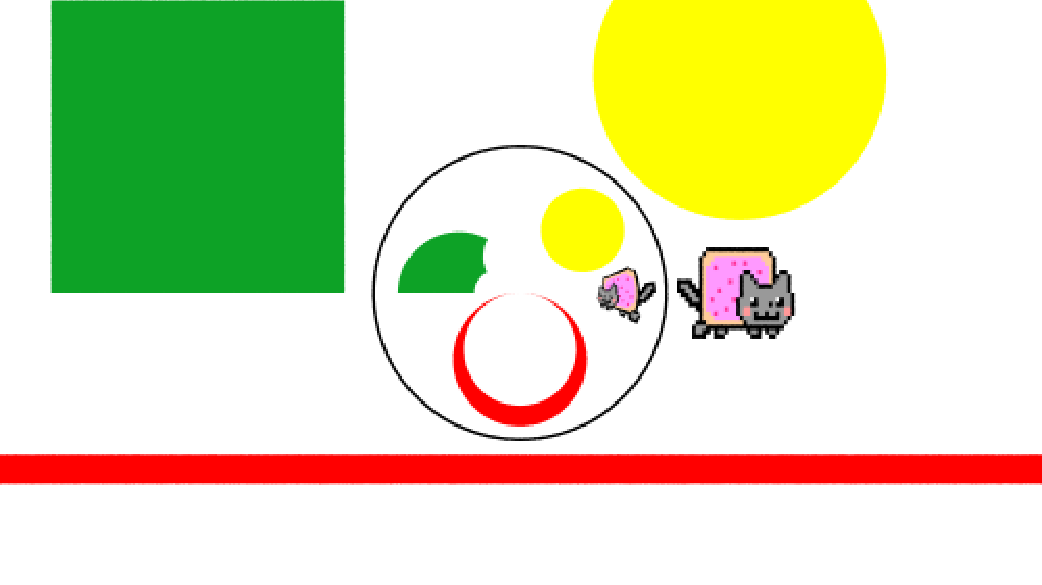
\includegraphics[width=3in, height=3in, keepaspectratio]{../img/klein/circleInversion.pdf}
    \caption{Circle Inversion}
    \label{fig:circleInversion}
 \end{center}
\end{figure}

\subsection{Stereographic Projection}

拡張複素平面はリーマン球面という名の通り, 球面で表すことで全
体をよく見ることができる.
地図の制作のため, 地球のような球面を平面に投影する方法が様々に考えられて
きたが, 複素平面を球面へと写像するためには, \emph{立体射影}({\it
stereographic projection})と呼ばれる方法がよく使われる.
立体射影は角度と円を保つため, メビウス変換と相性が良い.

ある球面上の点をPとおくと, Pを立体射影で移した複素平面上の像は球面の北極
からPへと引いた直線と複素平面との交点となる.
図\ref{fig:stereoProject}は立体射影を図示したものである.
赤の円は単位円を表す. 単位円は赤道へと移る.

Saul Schleimer, Henry Segermanはこれを利用した全天球画像へのエフェクトを
考案している\cite{spherical}.
図\ref{fig:spherical}は正距円筒図法(Equirectangular map)と球の内側からみ
た視点と, 複素平面とリーマン球面を可視化したものである.
このように, 複素平面上での回転は球の回転として表わすことができる.
\footnote{Spherical Droste video: \url{https://www.youtube.com/watch?v=qvh-EAipIUk\&t=4s}}

\begin{figure}[htbp]
 \center
 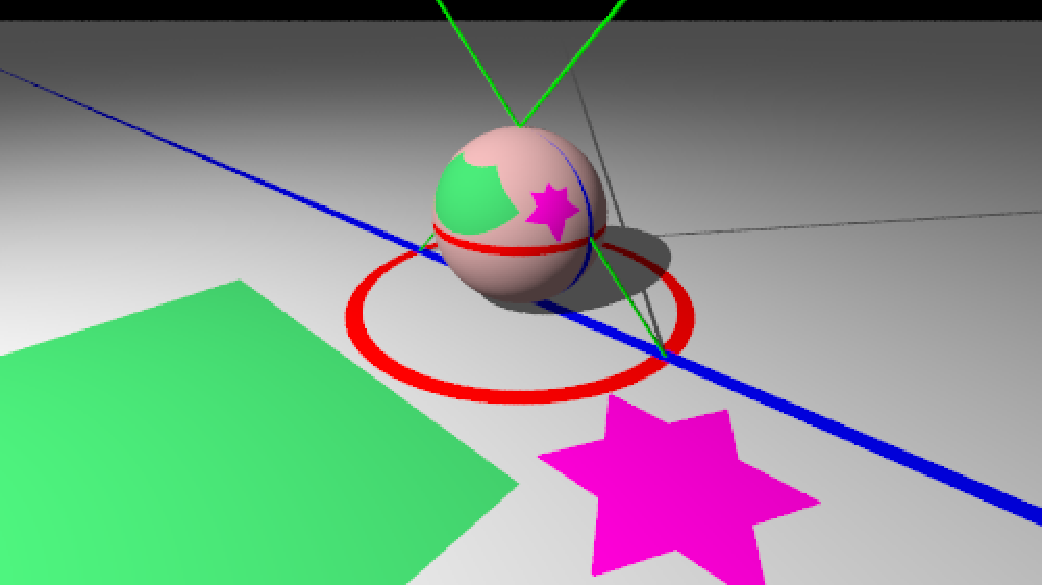
\includegraphics[width=3in, height=3in, keepaspectratio]{../img/klein/stereoProject.pdf}
 \caption{Stereographic Projection}
 \label{fig:stereoProject}
\end{figure}

\begin{figure}[htbp]
 \begin{minipage}{0.5\hsize}
  \center
  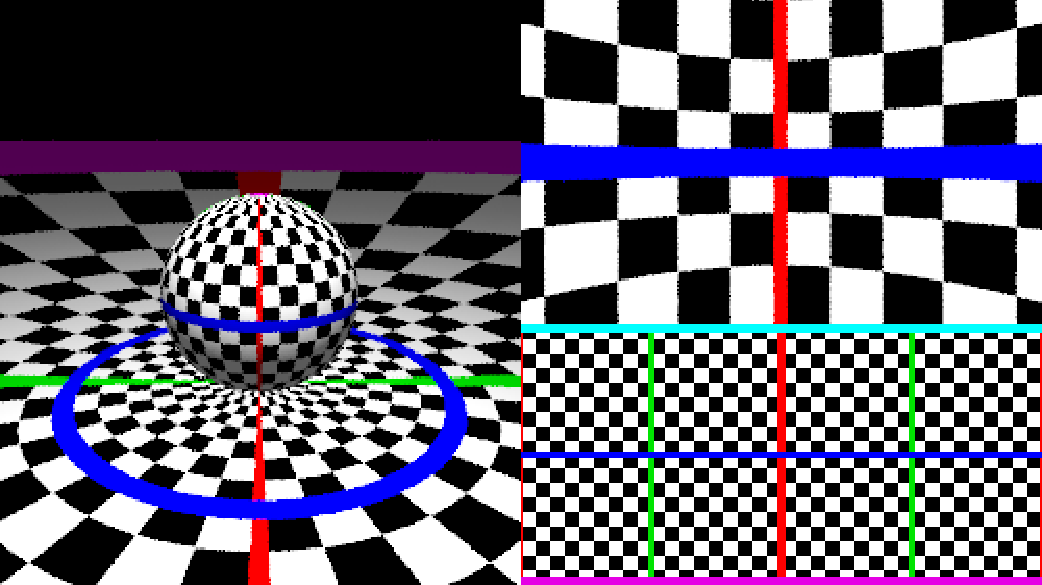
\includegraphics[width=3in, height=3in, keepaspectratio]{../img/klein/spherical.pdf}
  \subcaption{Stereographic }
  \label{fig:sphericalStandard}
 \end{minipage}
 \begin{minipage}{0.5\hsize}
  \center
  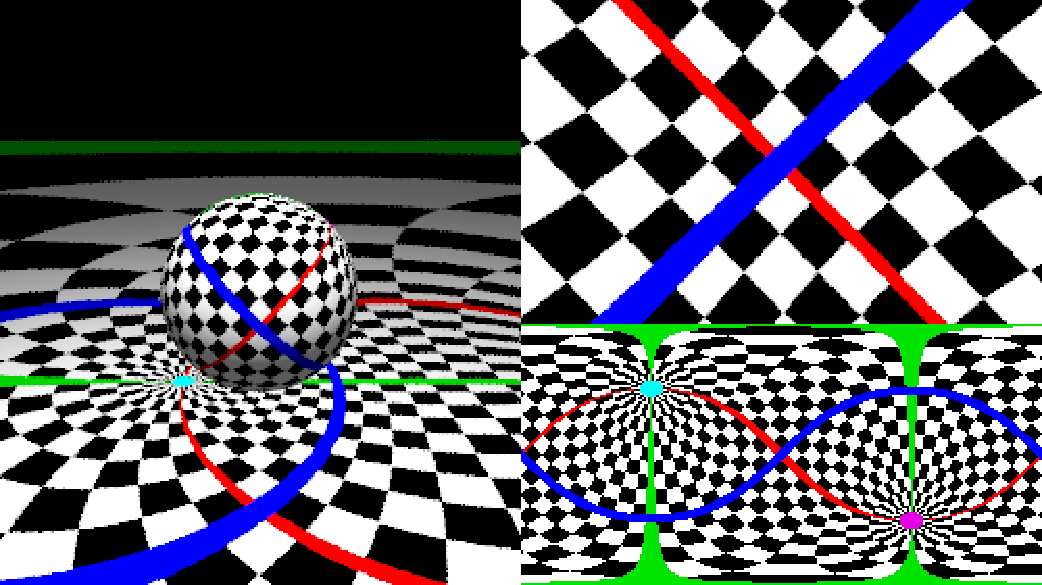
\includegraphics[width=3in, height=3in, keepaspectratio]{../img/klein/sphericalRotation.pdf}
  \subcaption{Stereographic 2}
  \label{fig:sphericalRotation}
 \end{minipage}
 \caption{Spherical image}
 \label{fig:spherical}
\end{figure}

\subsection{Graph Traversal Approach}

この節では木構造の探索によるクライン群の可視化について記述する.
群を構成する変換の全組み合わせを調べるとき,変換の語で構成される木構造を考える.
図\ref{fig:wordTree}のような木はケーリーグラフ(Cayley graph)と呼ばれ4種類の変換の合成の組合せを表わしている.
この木を探索することで得られる合成変換を用いて群の作用を可視化する.
疑似コードを含む詳細な解説は『インドラの真珠』にある.

メビウス変換は4つの複素数で構成されているが, このままでは自由度が高すぎ
るため,群を考えるときにはパラメータ化する.
パラメータ化された式は群の「レシピ」ともよばれる.
例えば, 『インドラの真珠』で使われる「おばあちゃんのレシピ」では, 二つの複素数
$t_a, t_b$をパラメータにとることで, 以下のように2つの生成元を得ることができる.
\begin{align*}
 t_a, t_b \in \mathbb{C} \\
 x^2 - t_a t_b x + t_a^2 + t_b^2 = 0 \text{の一方の解}x\text{を}t_{ab} = x \text{とする. }\\
 z_0 = \frac{(t_{ab} -2)t_b}{t_b t_{ab} - 2 t_a + 2it_{ab}}\\
 A = \left(
      \begin{array}{ccc}
       \frac{t_a}{2} & \frac{t_a t_{ab} - 2 t_b + 4i}{(2 t_{ab} + 4)z_0} \\
       \frac{(t_a t_{ab} - 2 t_b -4i)z_0}{2 t_{ab} - 4} & \frac{t_a}{2}
      \end{array}
     \right)
 B = \left(
      \begin{array}{ccc}
       \frac{t_b - 2i}{2} & \frac{t_b}{2} \\
       \frac{t_b}{2} & \frac{t_b + 2i}{2}
      \end{array}
     \right)
\end{align*}
「おばあちゃんのレシピ」は群を可視化した際に綺麗な図がレンダリングされるように調整がなされている.

\begin{figure}[htbp]
 \center
 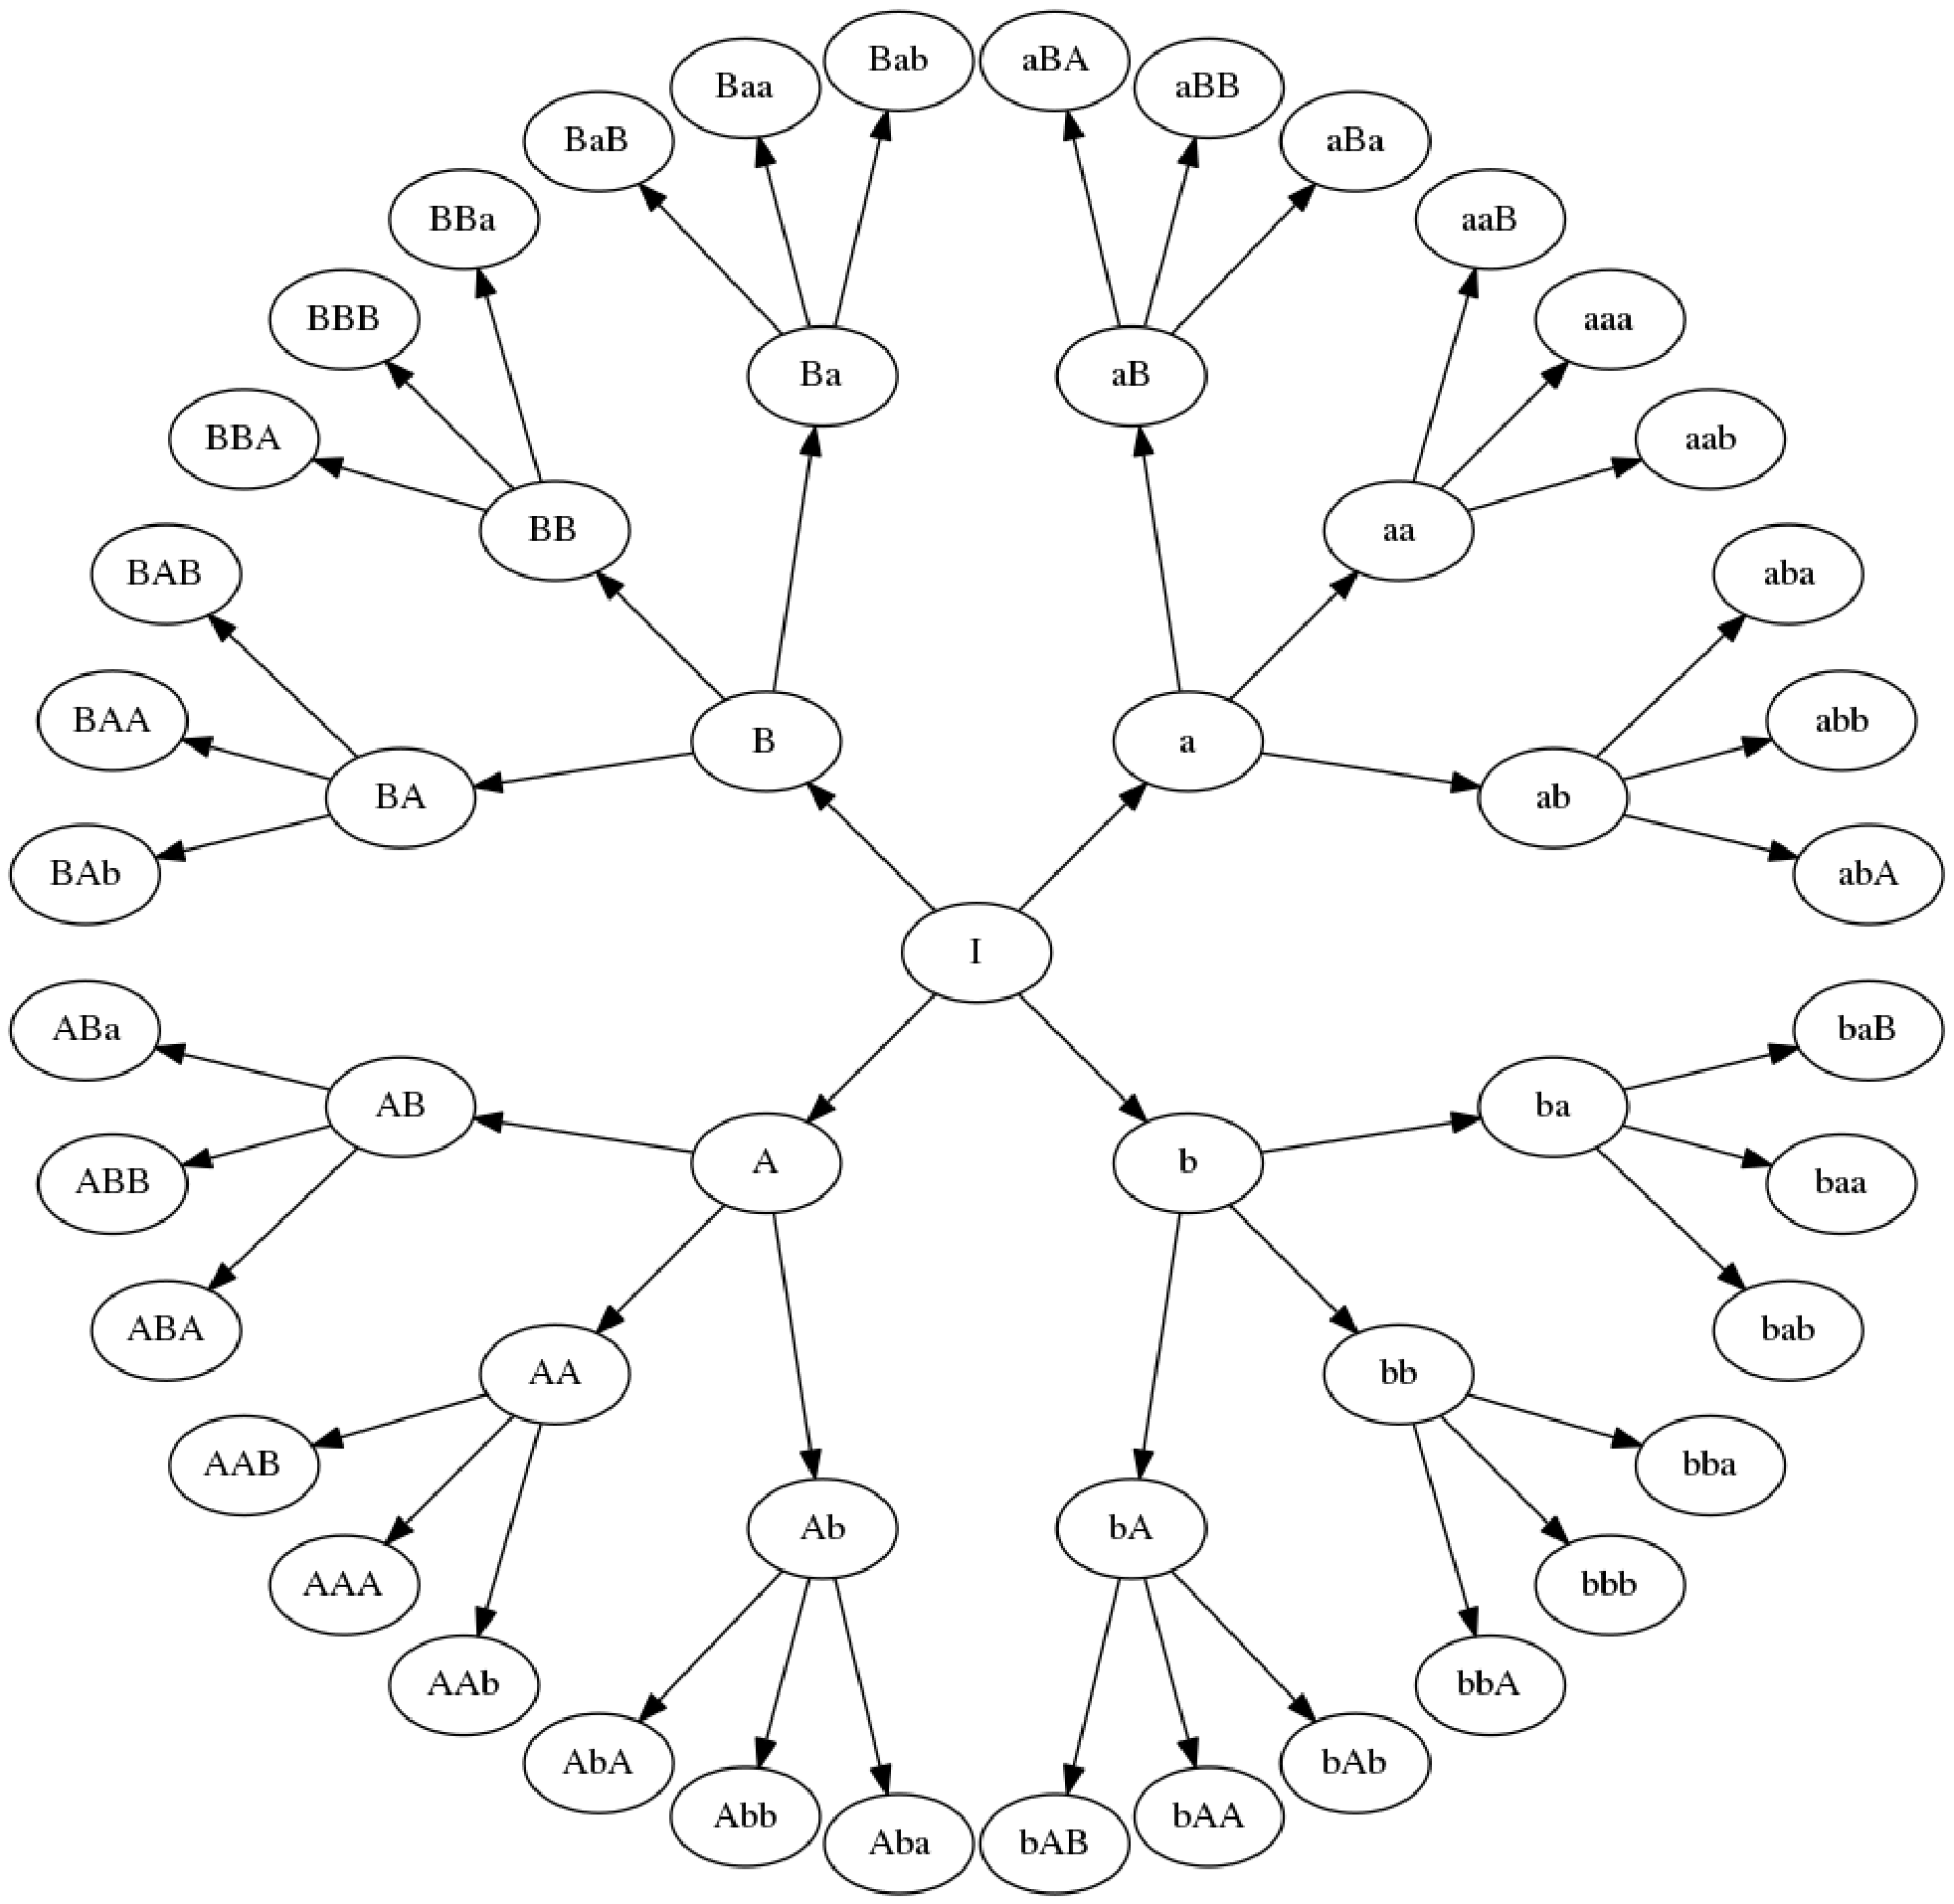
\includegraphics[width=3in, height=3in, keepaspectratio]{../img/klein/wordTree.pdf}
 \caption{Word Tree}
 \label{fig:wordTree}
\end{figure}

\subsubsection{Rendering the Orbit of Transformations}

まず, 円の反転で構成される群を可視化してみよう.
円の反転は変換自体を円という図形で表現できるため, その作用を理解しやすい.
図\ref{fig:schottky}には4つ円の内側にたくさんの円が描かれている.

外側にある4つの大きな円を反転円とよぶ.
それぞれの反転円の反転は自分以外の反転円を自分の内側に移す.
よって,それぞれの反転円に関する反転を行なうと, それぞれの円の内側には3
つの円が移され,合せて12個の小円ができる.
新たにできた小円に対してもその小円が属している反転円以外の反転を適用することで, 小円の下に新たな小円ができる.
このことを繰り返すと,図\ref{fig:schottky}のように,円が入れ子状につらな
る図を得ることができる.
これを反転円の\emph{軌道}とよぶ.
また,円列の極限を極限集合とよぶ.

図\ref{fig:schottky}では反転円の軌道を描いが, 同様にして違う図形の軌道を描くこともできる.
例えば, 図\ref{fig:orbit}は中央に置いた猫の画像を4つ反転円による反転で移した軌道を描いた.

このアルゴリズムは変換で構成される木構造を幅優先探索で探索することに等しい.
例えば, 図\ref{fig:wordTree}の語の木を時計回りに探索すると$a, b, A, B,
aB, aa, ab, ba, bb, ...$の順に合成された変換を得ることができる.
あらかじめ決められた深さまで調べたら, 得られたすべての変換の語を大本とな
る図形(図\ref{fig:orbit}における中央の猫)に対して作用させることで, おお
まかに生成元の作用を調べることができる.

\begin{figure}[htbp]
 \begin{minipage}{0.49\hsize}
  \begin{center}
   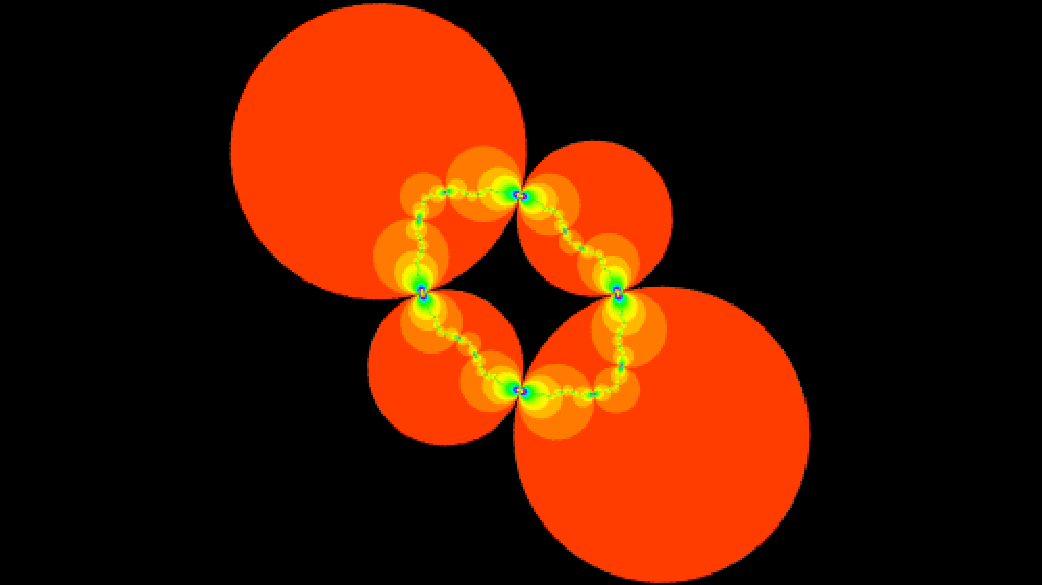
\includegraphics[width=3in, height=3in, keepaspectratio]{../img/klein/schottkyCircles.pdf}
   \caption{Schottky Circles}
   \label{fig:schottky}
  \end{center}
 \end{minipage}
 \begin{minipage}{0.49\hsize}
  \begin{center}
   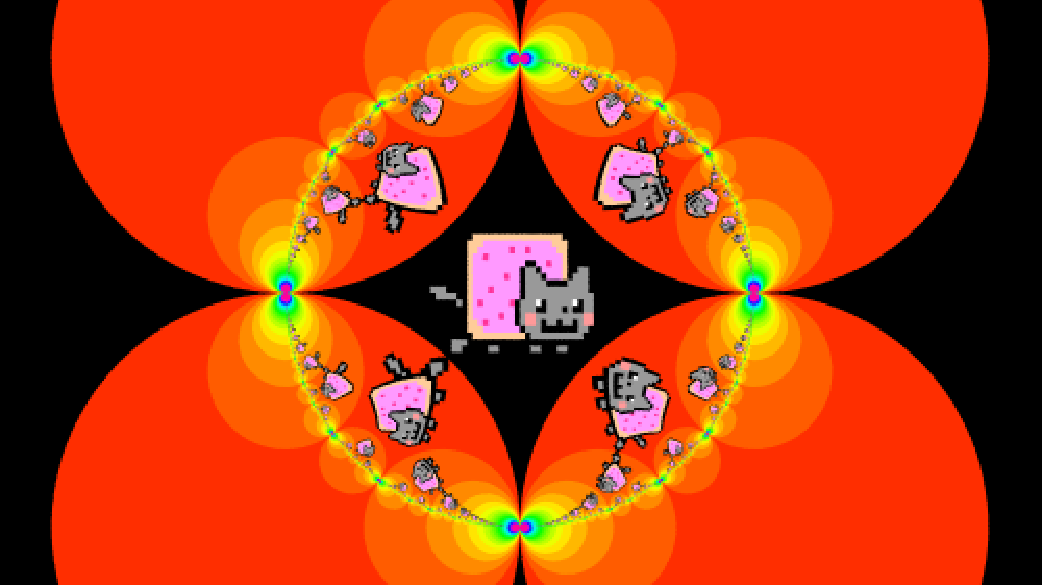
\includegraphics[width=3in, height=3in, keepaspectratio]{../img/klein/circleOrbit.pdf}
   \caption{orbit}
   \label{fig:orbit}
  \end{center}
 \end{minipage}
\end{figure}


\subsubsection{Rendering the Limit Set}

より複雑なメビウス変換群を可視化する際には, 極限集合を直接描く方法が使わ
れる.
極限集合はケーリーグラフにおいて, 無限の深さの語に対応している.
しかし, 現実にそれを求めることは不可能なので, 群の生成元の固定点をある程
度の長さをもった変換の語で移すことで求める.
例えば, 変換$a$の固定点は任意の点に$a$を繰り返し適用した点, つまり
$\overline{a}$を適用した極限点と考えることができる.
例えば, 変換$abbAAb\overline{a}$で表わされる極限点は$a$の固定点を合成変換$abbAAb$で移すことで求めることができる.
この時, $abbAAb$を接頭語と呼ぶ.

図\ref{fig:wordTree}の語の木を時計回りに長さ3までの語を探索すると,$ aBA, aBB, aBa, aaB, ...$という順で接頭語が得られる.
これらの語に, 逆変換をかけないように, 生成元の固定点を与えると極限点を求めることができる.
例えば$aBA$を用いて$\overline{A}, \overline{b}, \overline{B}$の3つの固定点を変換すると互いに近い3つの極限点が得られる.
$aab\overline{a}$と$aaa\overline{a}$のように隣同士の接頭語を持つ極限点や
$aaa\overline{a}$と$aaa\overline{b}$のような同じ接頭語を持つ極限点同士は
近い.
そのため, 得られた点同士を順番に結ぶと図のようなフラクタル構造を持つ曲線を得ることができる.
実際に実装する場合には, 得られた点同士の距離によってより深い語への探索の打ち切りと継続を決める.

図\ref{fig:apr}はP.Nylander氏による作品\footnote{bugman123.com Fractals:
\url{http://bugman123.com/Fractals/index.html}}を参考に描画した.
中央右側の蝶をおばあちゃんのレシピで得られた群の生成元で移した.
虹色の曲線は極限集合である.
どちらの図も図形の軌道は最終的に極限集合へと収束していくことがわかる.

ただし, 綺麗に描画するには様々な工夫が必要となる.
まず, 放物型変換は固定点への収束に時間がかかため, 放物型変換の固定点付近
をうまく描画するためには, 放物型の生成元のための特別な処理が必要である.
図\ref{fig:apr}の右端をよく見ると直線で結ばれていることがわかる.
ここには放物型変換の固定点が存在しており, 収束が遅いため, この近辺の極限点を得るためには, より長い接頭語が必要となっている.
インドラの真珠では特殊語アルゴリズムと呼ばれるアルゴリズムでこの問題に対処する.

また, ある変換に対してその逆変換をかけてしまうと元にもどってしまうことは
自明であるが, 特定の変換の組み合わせが逆戻りを生み出してしまうことがある.
例えば, 先に述べた平行移動の例において,abABという変換は点を一周させて元の場所に戻してしまう.
このような変換をもたない群を\emph{自由群}と呼ぶ.
効率よく描画するためには,うまくこのような元を取り除く必要がある.これを解決するためには有限オートマトンが使われる.
インドラの真珠においても有限オートマトンの使い方に関する解説はあるが, よ
り数学的な事項は『Word Processing In Groups』\cite{wordProcessing}が詳し
い.

先に述べたように,メビウス変換の群すべてがクライン群になるわけではない.
群のレシピのパラメータの中には描画すると極限集合が収束せず,図
\ref{fig:non-discrete}のように乱れるようなものがある.
このような群は\emph{非離散群}と呼ばれ,クライン群ではない.
この離散と非離散のパラメータ領域を描画した図は\emph{スライス}と呼ばれ,
スライスの離散と非離散の境界もフラクタル形状となる.
境界付近のパラメータを用いて描画するとしばしば極限集合が興味深い形になる.
山下靖氏のページ\footnote{Discreteness Locus:
\url{http://vivaldi.ics.nara-wu.ac.jp/~yamasita/Slice/}}では様々なスライ
スを見ることができる.
どのようなパラメータが離散的であるか,すなわちクライン群となるかを調べることがクライン群の研究テーマの一つとなる.

\begin{figure}[h!tbp]
 \begin{subfigure}{0.49\hsize}
   \begin{center}
    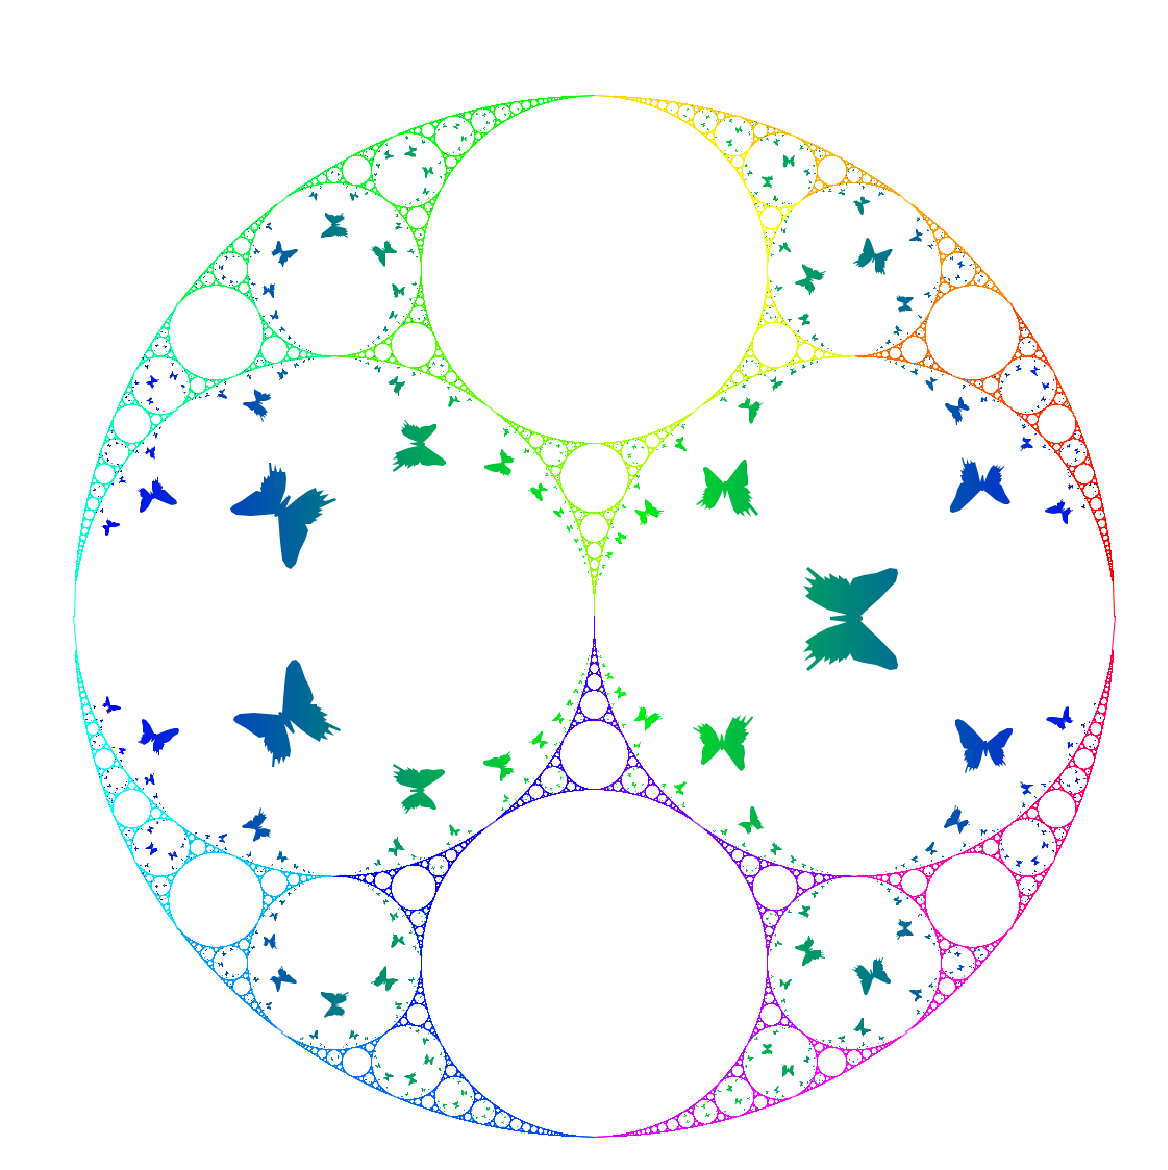
\includegraphics[width=3in, height=3in, keepaspectratio]{../img/klein/apr.pdf}
    \caption{}
    \label{fig:apr}
   \end{center}
 \end{subfigure}
 \hspace*{\fill}
 \begin{subfigure}{0.49\hsize}
   \begin{center}
    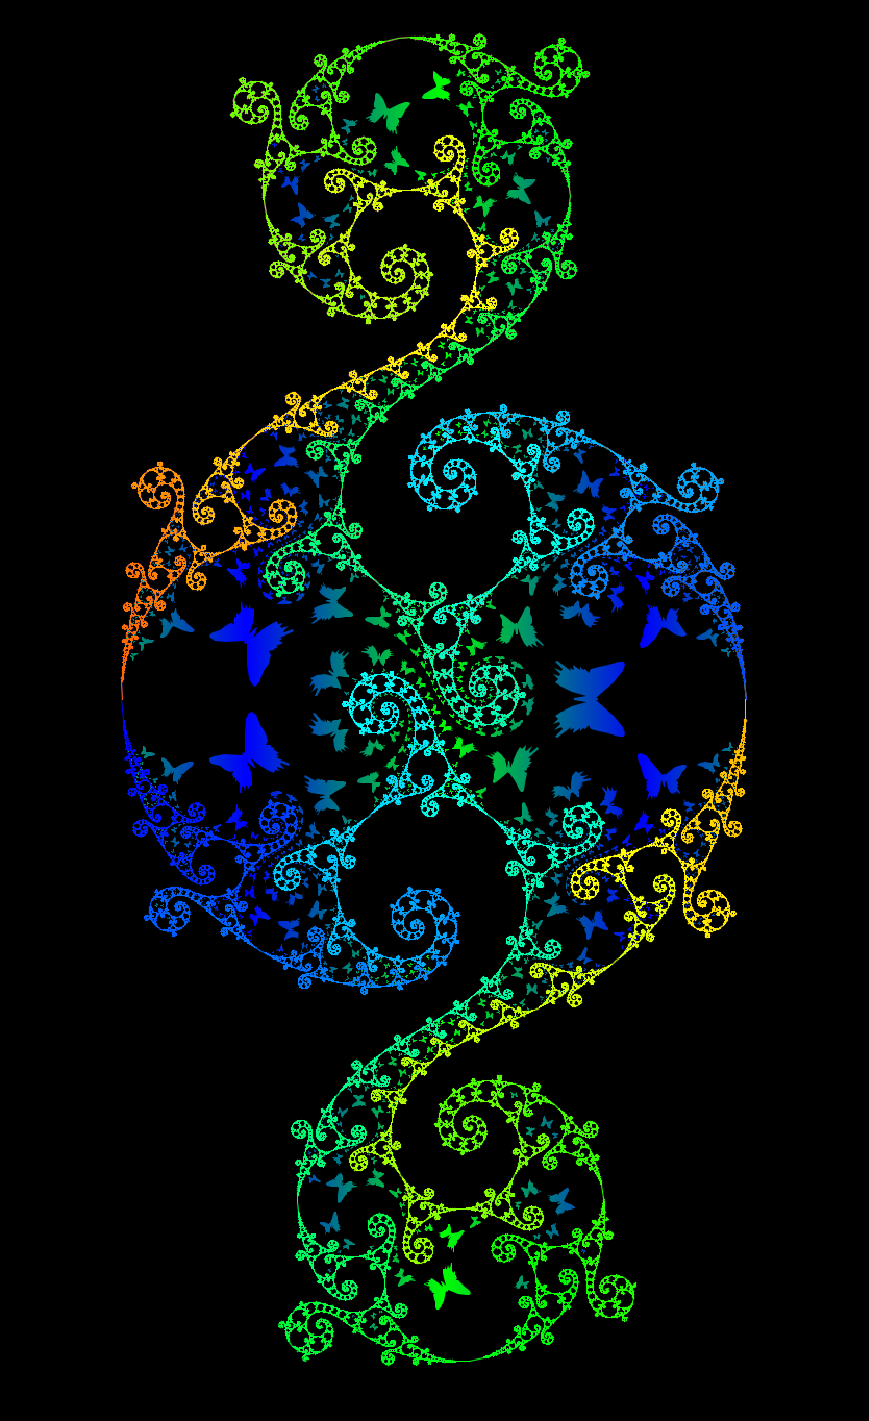
\includegraphics[width=3in, height=3in, keepaspectratio]{../img/klein/comp.pdf}
    \caption{}
    \label{fig:comp}
   \end{center}
 \end{subfigure}
 \caption{The limit set of Kleinian Groups}
 \label{fig:limitsetWithOrbit}
\end{figure}

\begin{figure}[htbp]
 \begin{subfigure}{0.49\hsize}
  \begin{center}
   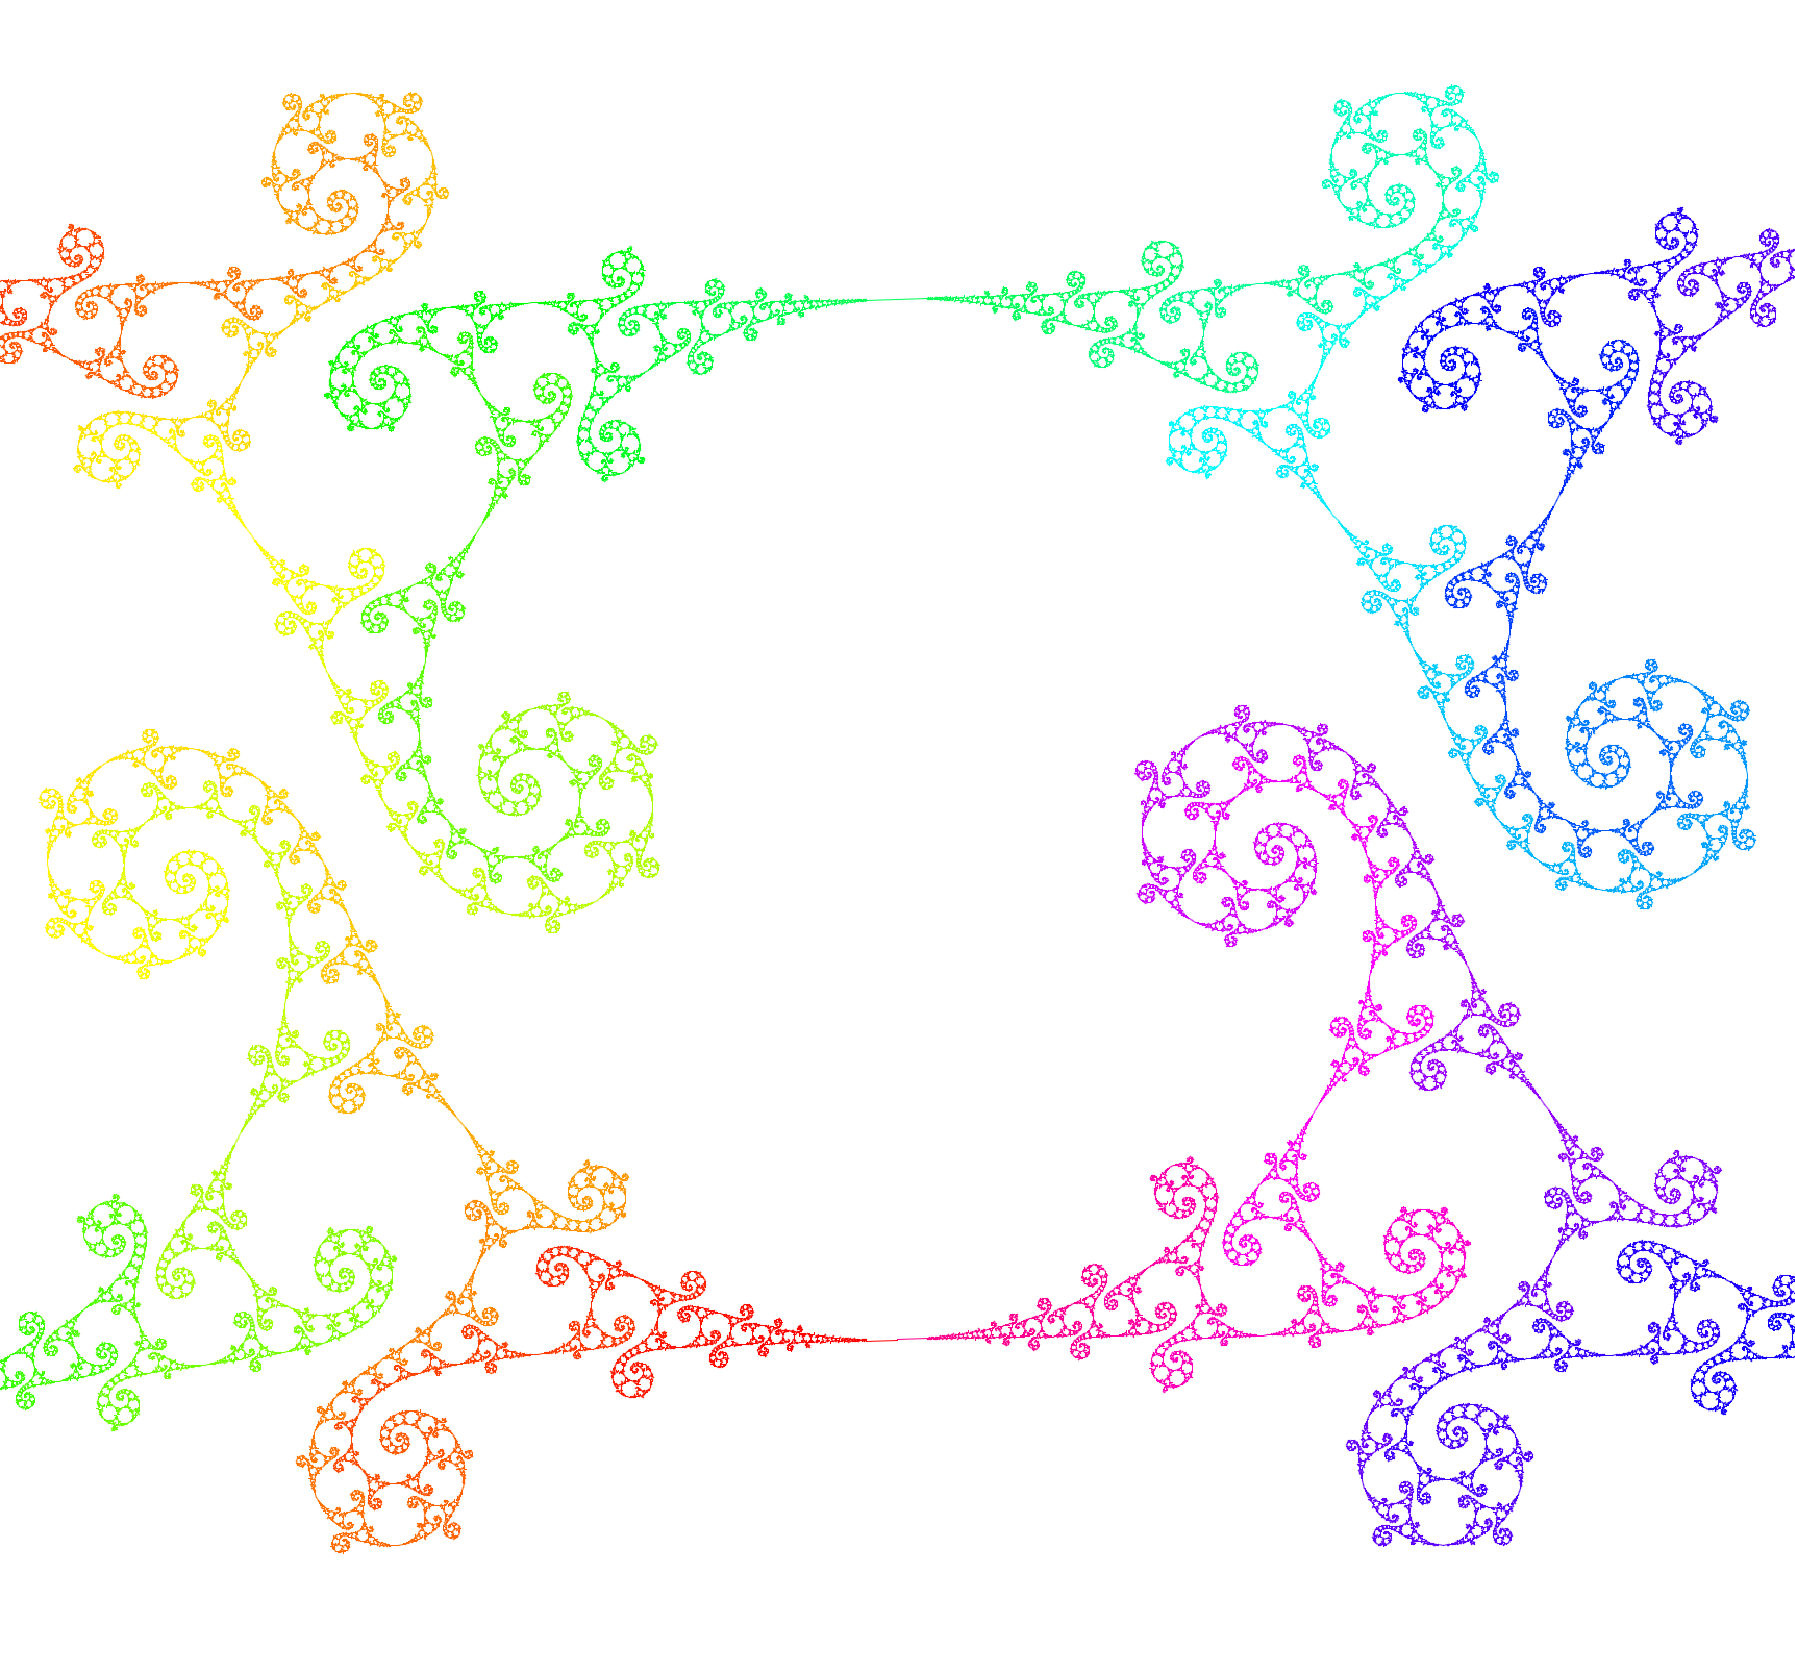
\includegraphics[width=3in, height=3in, keepaspectratio]{../img/klein/horizon.pdf}
   \caption{}
   \label{fig:horizon1}
  \end{center}
 \end{subfigure}
 \begin{subfigure}{0.49\hsize}
  \begin{center}
   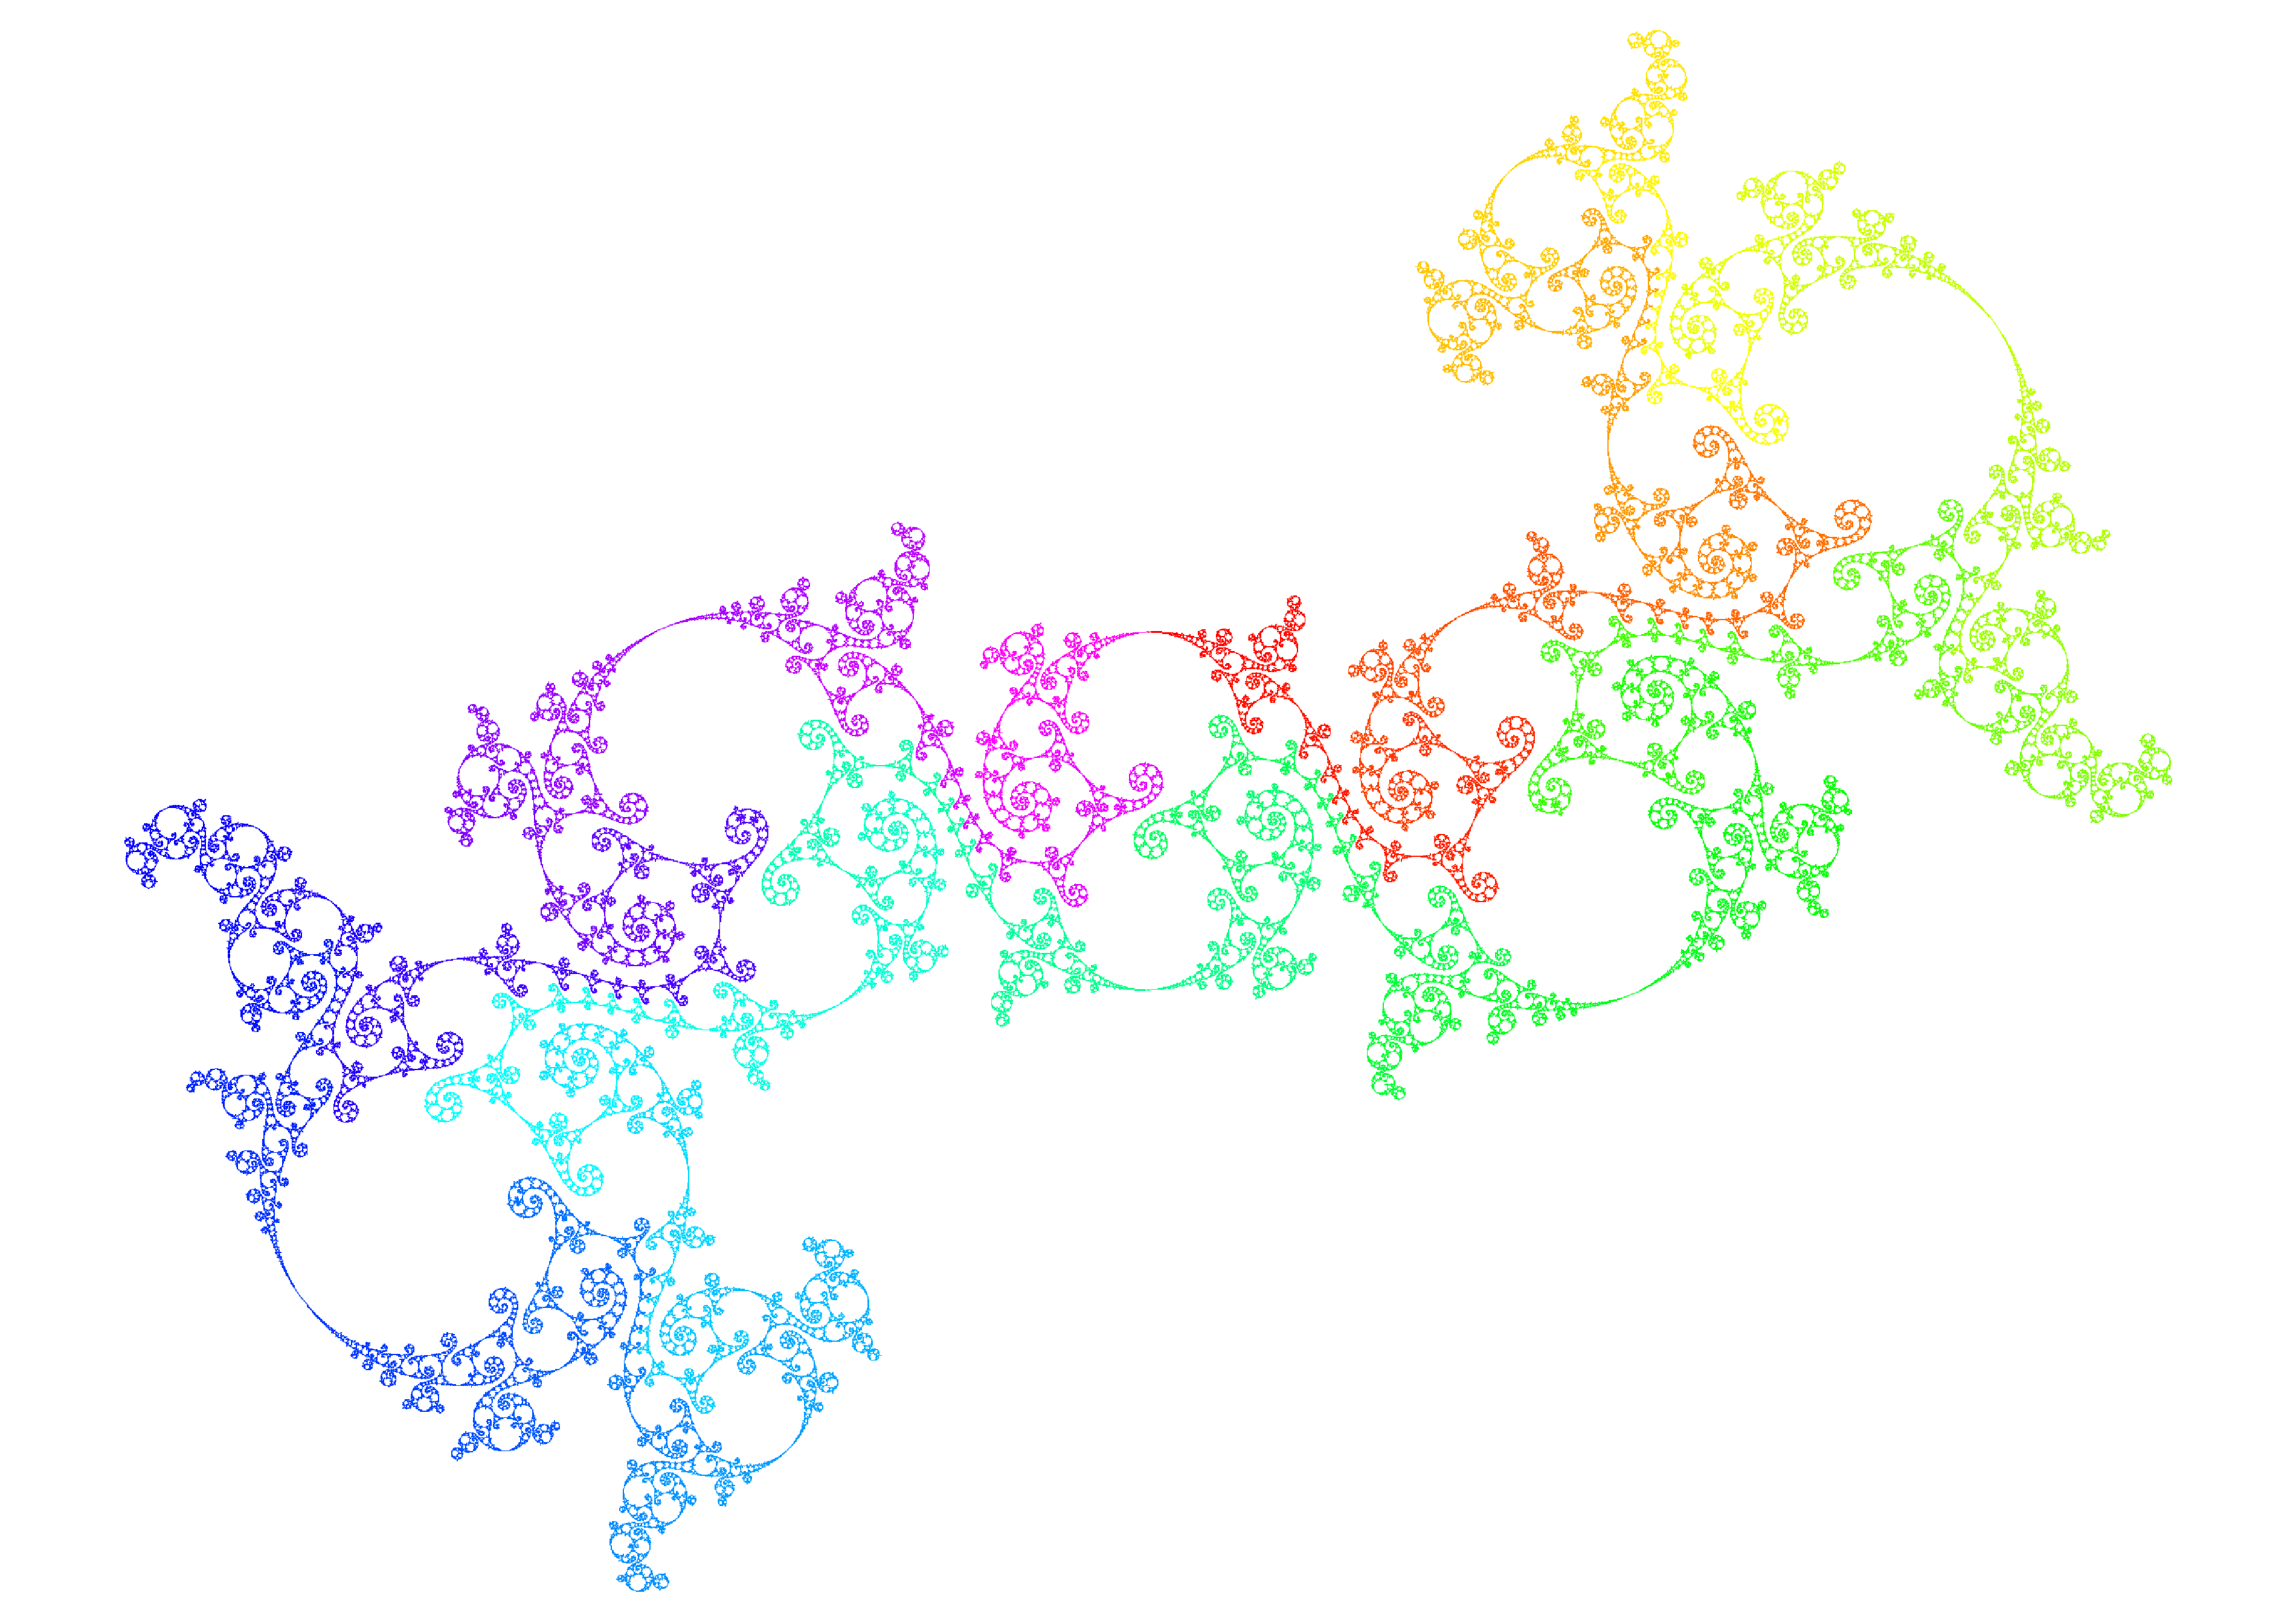
\includegraphics[width=3in, height=3in, keepaspectratio]{../img/klein/limit-horizontal.pdf}
   \caption{}
   \label{fig:horizon2}
  \end{center}
 \end{subfigure}\\
 \begin{subfigure}{0.49\hsize}
  \begin{center}
   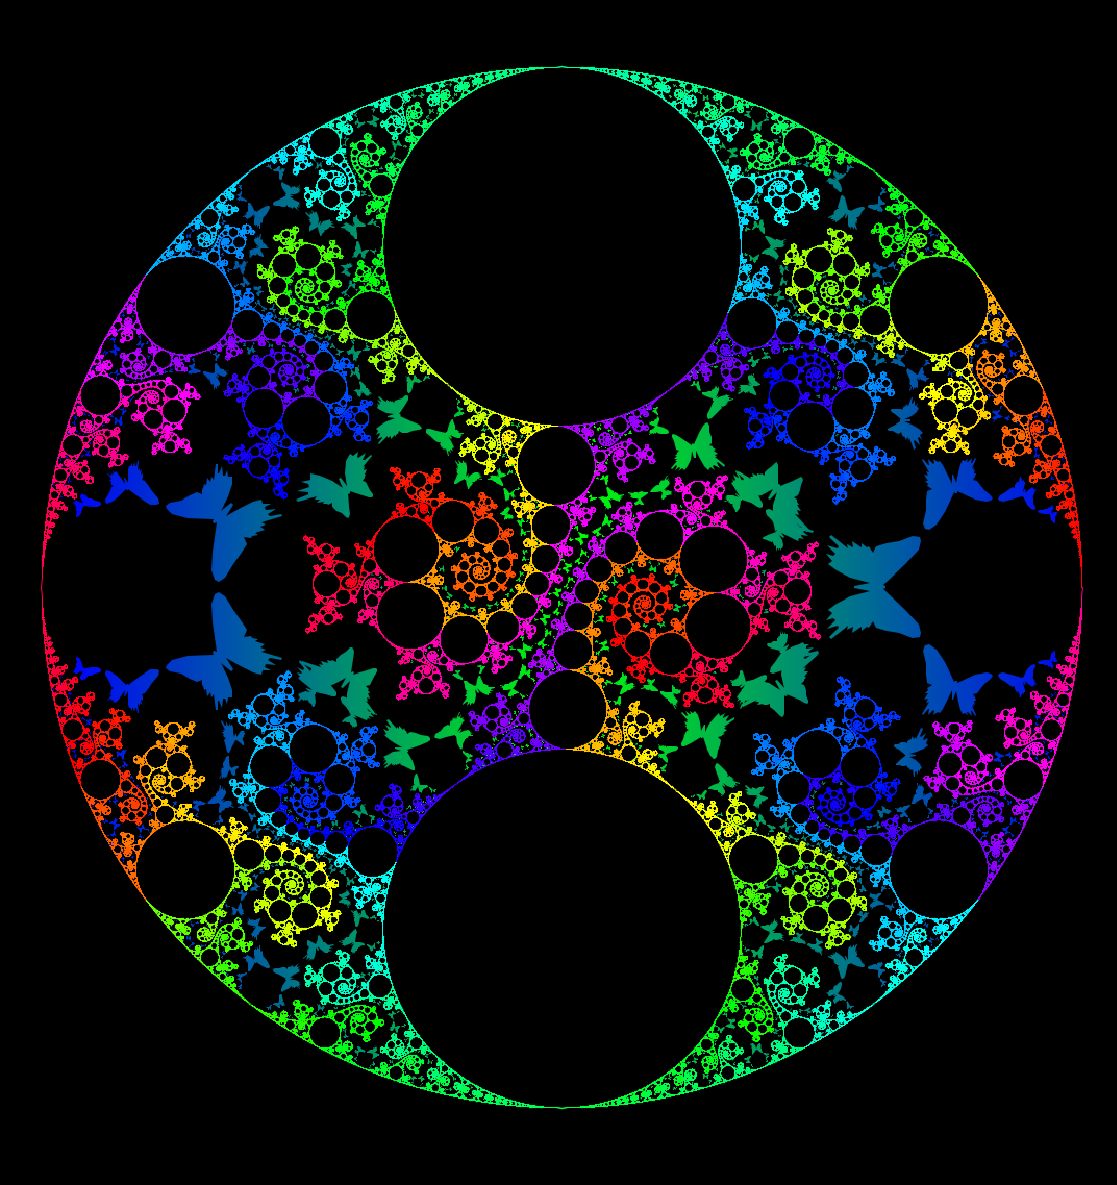
\includegraphics[width=3in, height=3in, keepaspectratio]{../img/klein/limit3.pdf}
   \caption{}
   \label{fig:limit3}
  \end{center}
 \end{subfigure}
 \begin{subfigure}{0.49\hsize}
  \begin{center}
   
\includegraphics[width=3in, height=3in, keepaspectratio]{../img/klein/limit4.pdf}
   \caption{}
   \label{fig:limit4}
  \end{center}
 \end{subfigure}
 \caption{The limit set of Kleinian Groups}
 \label{fig:limitset}
\end{figure}

\begin{figure}[htbp]
 \begin{center}
  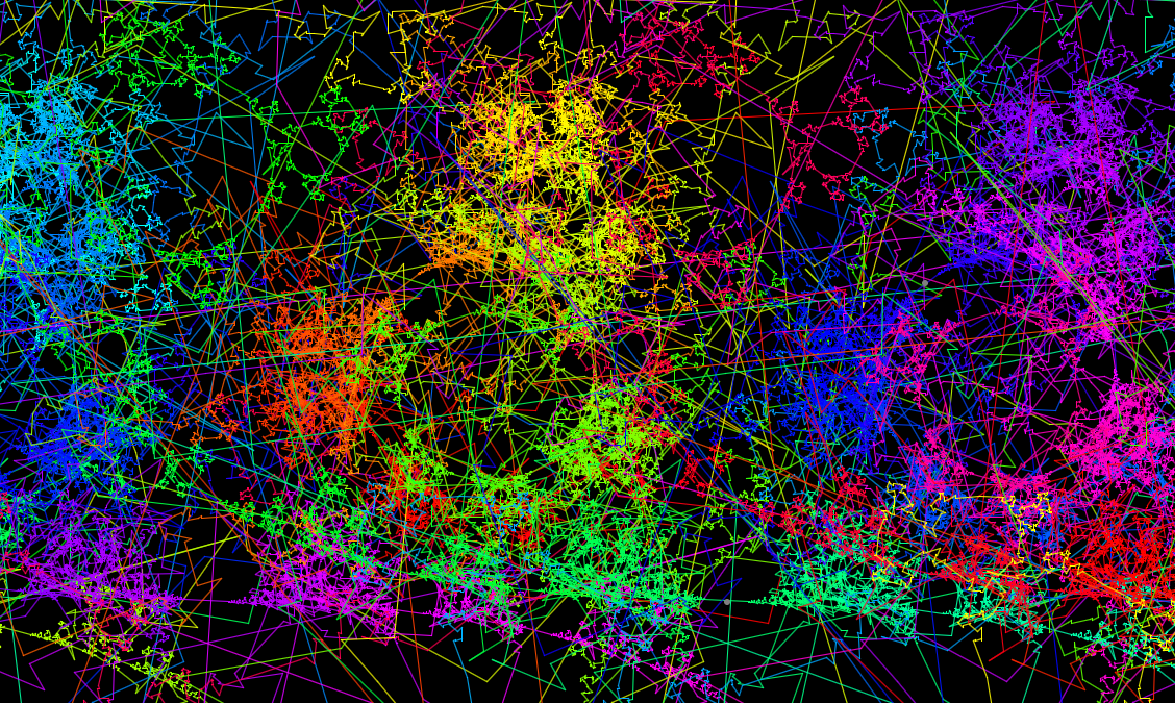
\includegraphics[ height=1.5in, keepaspectratio]{../img/klein/non-discrete.pdf}
  \caption{non discrete}
  \label{fig:non-discrete}
 \end{center}
\end{figure}

\subsubsection{Faults of Graph Traversal Approach}

グラフを探索する方法にはいくつかの欠点がある.
まず, 生成元や,探索を深くするごとに指数オーダーで計算量が増えてしまう.
また, 部分的に拡大したい場合に無駄な部分を計算しないといった処理にも手間
がかかる.
さらに木構造の探索は並列化に向かないため, 高速化が難しい.
そのため, 木構造の探索に頼らない方法がいくつか考案されている.

しかしながら, 最近のOpenCLやCUDAといった並列計算プラットフォームでは
Dynamic Parallelismという機能を用いることで,木構造探索の並列計算を行う
ことが可能である.
ただし, 最新のハードウェアに依存した機能のため, どの計算機環境でも使えるわけではない.

\subsection{Iterated Inversion System}

筆者らは, 1章でみたシェーダを用いたフラクタルのレンダリングアルゴリズム
に着想を得て, 円や球の反転で構成される群の軌道を高速に描画するためのアル
ゴリズム, \textit{Iterated Inversion System (IIS)}\cite{iis}を開発した.
円や球の座標と半径を直接計算するこれまでのアプローチに対して,このアルゴ
リズムは任意の点が属する円や球の深さを特定する.
これはスクリーンスペースのピクセルそれぞれに対して独立に計算することがで
きるのでGLSLによる並列計算,描画を行うことができる.

図\ref{fig:iis-orb}のような4つの反転円を考える.
黒い領域は基本領域とよぶ.
ある点がいずれかの円盤に属している時にその円に関する反転を行なう.
これを反転後の点がすべての円の外側に移されるまで繰り返す.
最終的に, 行なった反転の回数が, その点が属している円盤の深さとなる.
図\ref{fig:iis-orb}では青い点の軌道を描いている.
この点は二回反転が行なわれているので, 反転円から二番目の円に属している.
それぞれの計算はピクセルごとに行なうことができるため, 多項式時間で描画す
ることができる.
実際にこのアルゴリズムを用いてすべての点を基本領域へと移動させるためには,
無限回の反転が必要である. そのため, あらかじめ最大の反転回数を決めておく.

後に我々は単純な反転以外の生成元を導入する. 我々は基本領域にある点に対しては恒
等写像で, その他の点に対しては反転の合成を適用する写像$G$を考える.
より一般化した擬似コードをアルゴリズム\ref{iis2d}に示す.

 \begin{algorithm}
  \caption{Iterated Inversion System (IIS)}
  \label{iis2d}
  \begin{algorithmic}
   \REQUIRE count $= 0$ and coordinates $=$ position determined by
   pixel
   \FOR{$i=0$ to MAX\_INVERSION}
   \STATE inFundamentalDomain $\leftarrow$ \TRUE
   \FOR{ each map $G$ in Maps }
   \IF{$G$ is available to coordinates}
   \STATE coordinates $\leftarrow$ $G(\text{coordinates})$
   \STATE INCREMENT count
   \STATE inFundamentalDomain $\leftarrow$ \FALSE
   \ENDIF
   \ENDFOR
   \IF {inFundamentalDomain}
   \STATE BREAK for
   \ENDIF
   \ENDFOR
   \STATE RETURN count
  \end{algorithmic}
 \end{algorithm}

\begin{figure}[htbp]
 \center
 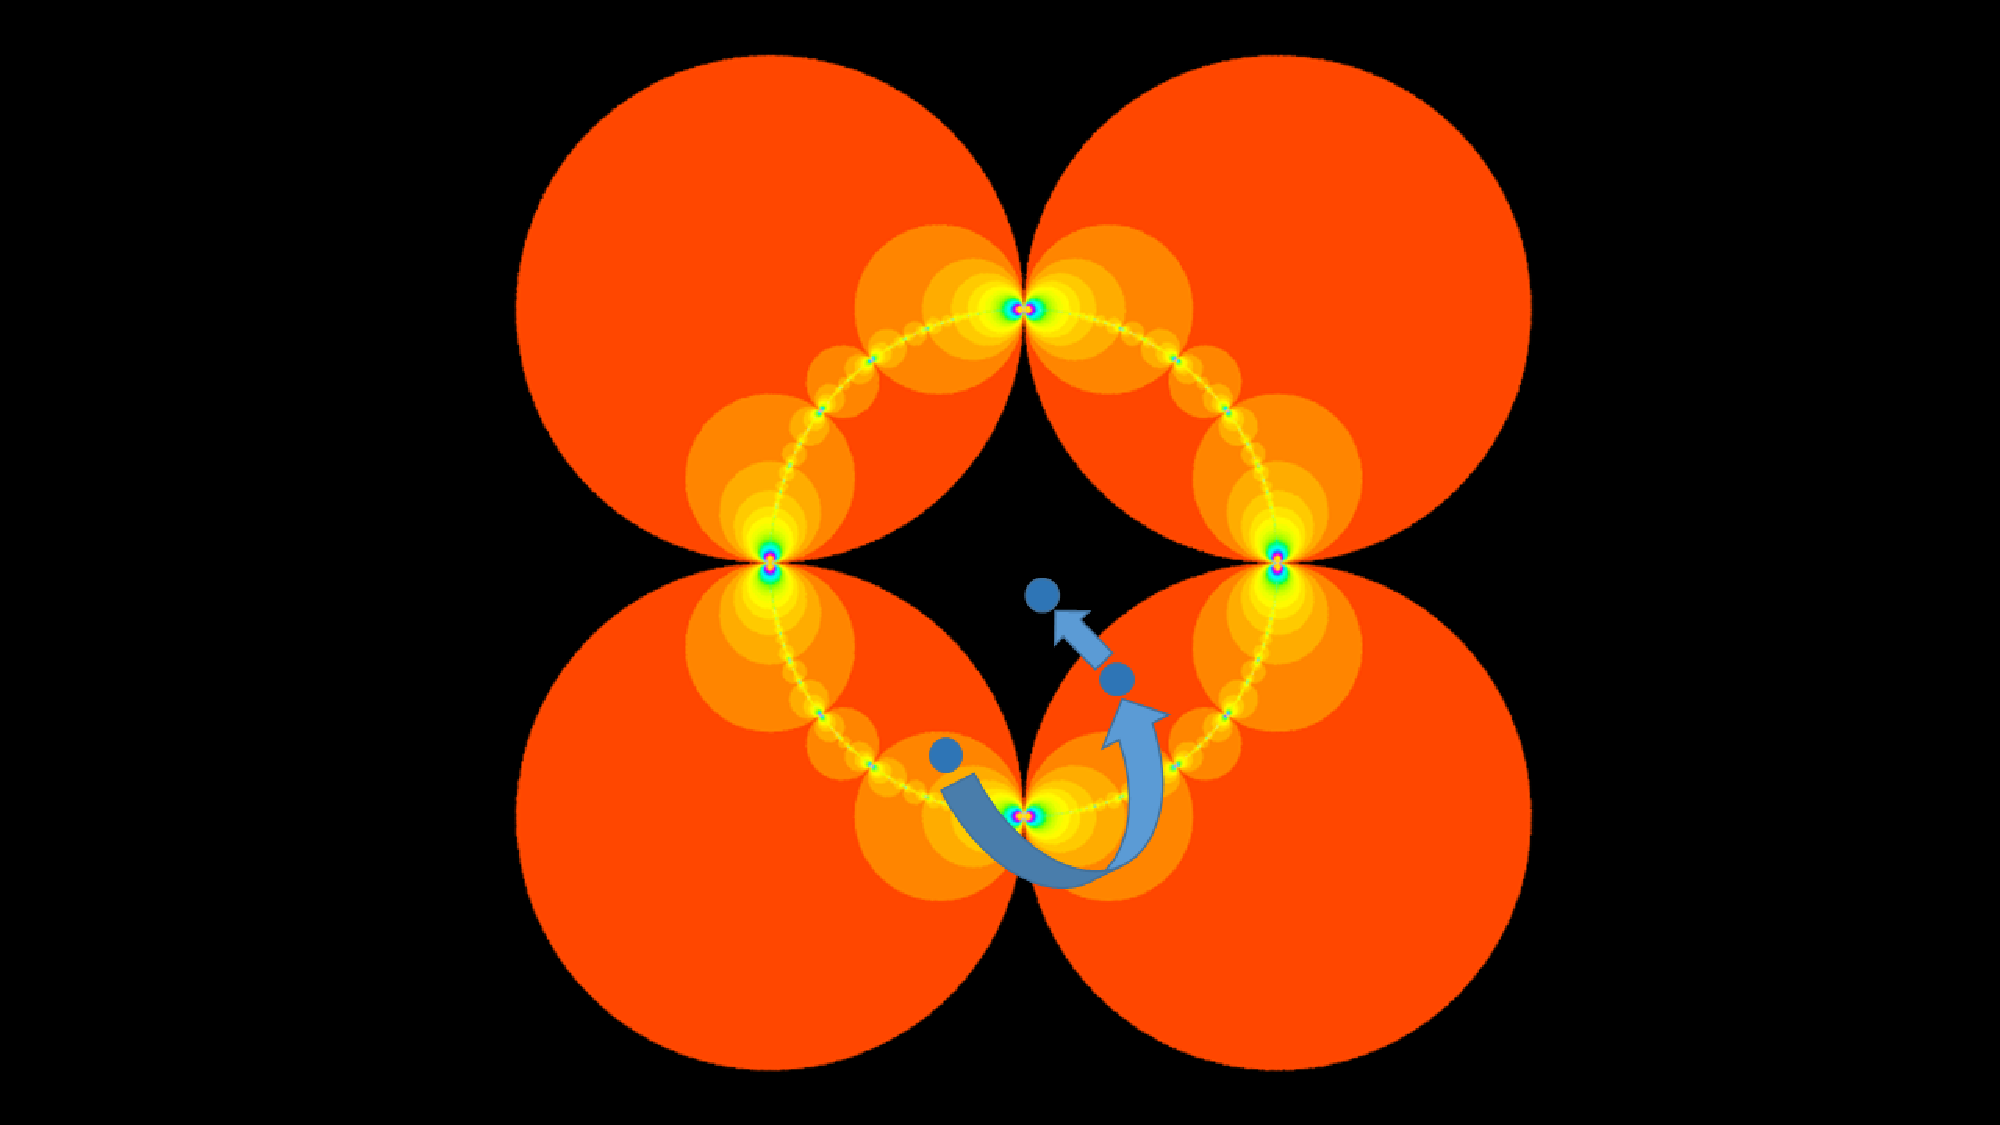
\includegraphics[ height=1.5in, keepaspectratio]{../img/klein/orb.pdf}
 \caption{Orbit}
 \label{fig:iis-orb}
\end{figure}

また, 球の反転による三次元形状もレイマーチングを用いることで, 高速に描画
することができる.
二次元の場合と同様に球の反転によるショットキー球の軌道を描こうとすると,
軌道はショットキー球の内側に連なってしまい, 描画に手間がかかる.
そこで我々は軌道の元となる球を用意し, その球をショットキー球の反転で移し
た軌道を描画する.
図\ref{fig:simpleGen3d}における灰色の球を\emph{ショットキー球},緑色の球を\emph{基本球}とよぶ.
基球をすべてのショットキー球の反転で移すと図\ref{fig:simpleOrb3d}のよう
な軌道が得られる.
レイマーチングに用いる距離関数を求めるため,
ここで簡単のために, 図\ref{fig:xySlice}に示されるような図
\ref{fig:iis-orb}のXY平面での断面を考えることにする.
橙色の円列はショットキー球の軌道, 水色の円が基本球の軌道である.
緑色の点$P2$はレイの先端, であるとすると最も近い球は$S2$となる.
しかし, 我々は$S2$の位置と半径は分からない.
基本球である$S1$の位置と半径のみを知っている.
そこで我々は変換のヤコビアンを用いて, 距離を逆算する.
ショットキー球の中心を$S$その半径を$R$,半径を適用する前の点を$P$とおくと
球の反転のヤコビアンは以下のように計算できる.
$ Jacobian = R^2 / distance(P, S)^2 $
また, 半径が無限大の球の反転のヤコビアンは1であることに注意する.
反転のヤコビアンを反転をおこなう毎にかけあわせていく.
最終的に近似されたレイの先端から最も近い球との距離は, 基本球と基本領域に
落ちた点との距離をヤコビアンの積で割ることで求めることができる.

この近似は荒いため, もう一つ考慮すべき事がある.
レイの先端が極限集合の外側にあるとき, その点は円の反転によって外側に移さ
れるため, レイは予期せずしてオブジェクトと突きぬけてしまう.
このことは図\ref{fig:artifact}のような乱れを生みだしてしまう.
オブジェクトの前面が正しくレンダリングされていない.
このような不具合を避けるため, 算出された距離を縮小する必要がある.
縮小率は球の大きさによって実験的に決めた.
擬似コードはアルゴリズム\ref{iis3d}に示した.

基本球の数を増やすことも可能である. 図\ref{fig:3baseSphere}は3つの基本球
の軌道を描画した.
基本球の大きさを変更することで, 形状を変形することができる.
図\ref{fig:limitSetOnSphere}は基本球の大きさを極限集合と同じ大きさにしたものである.
球の上に極限集合が描画されていることがわかる.

\begin{figure}[htbp]
 \begin{minipage}[b]{0.5\hsize}
  \begin{minipage}[]{0.49\hsize}
   \center
   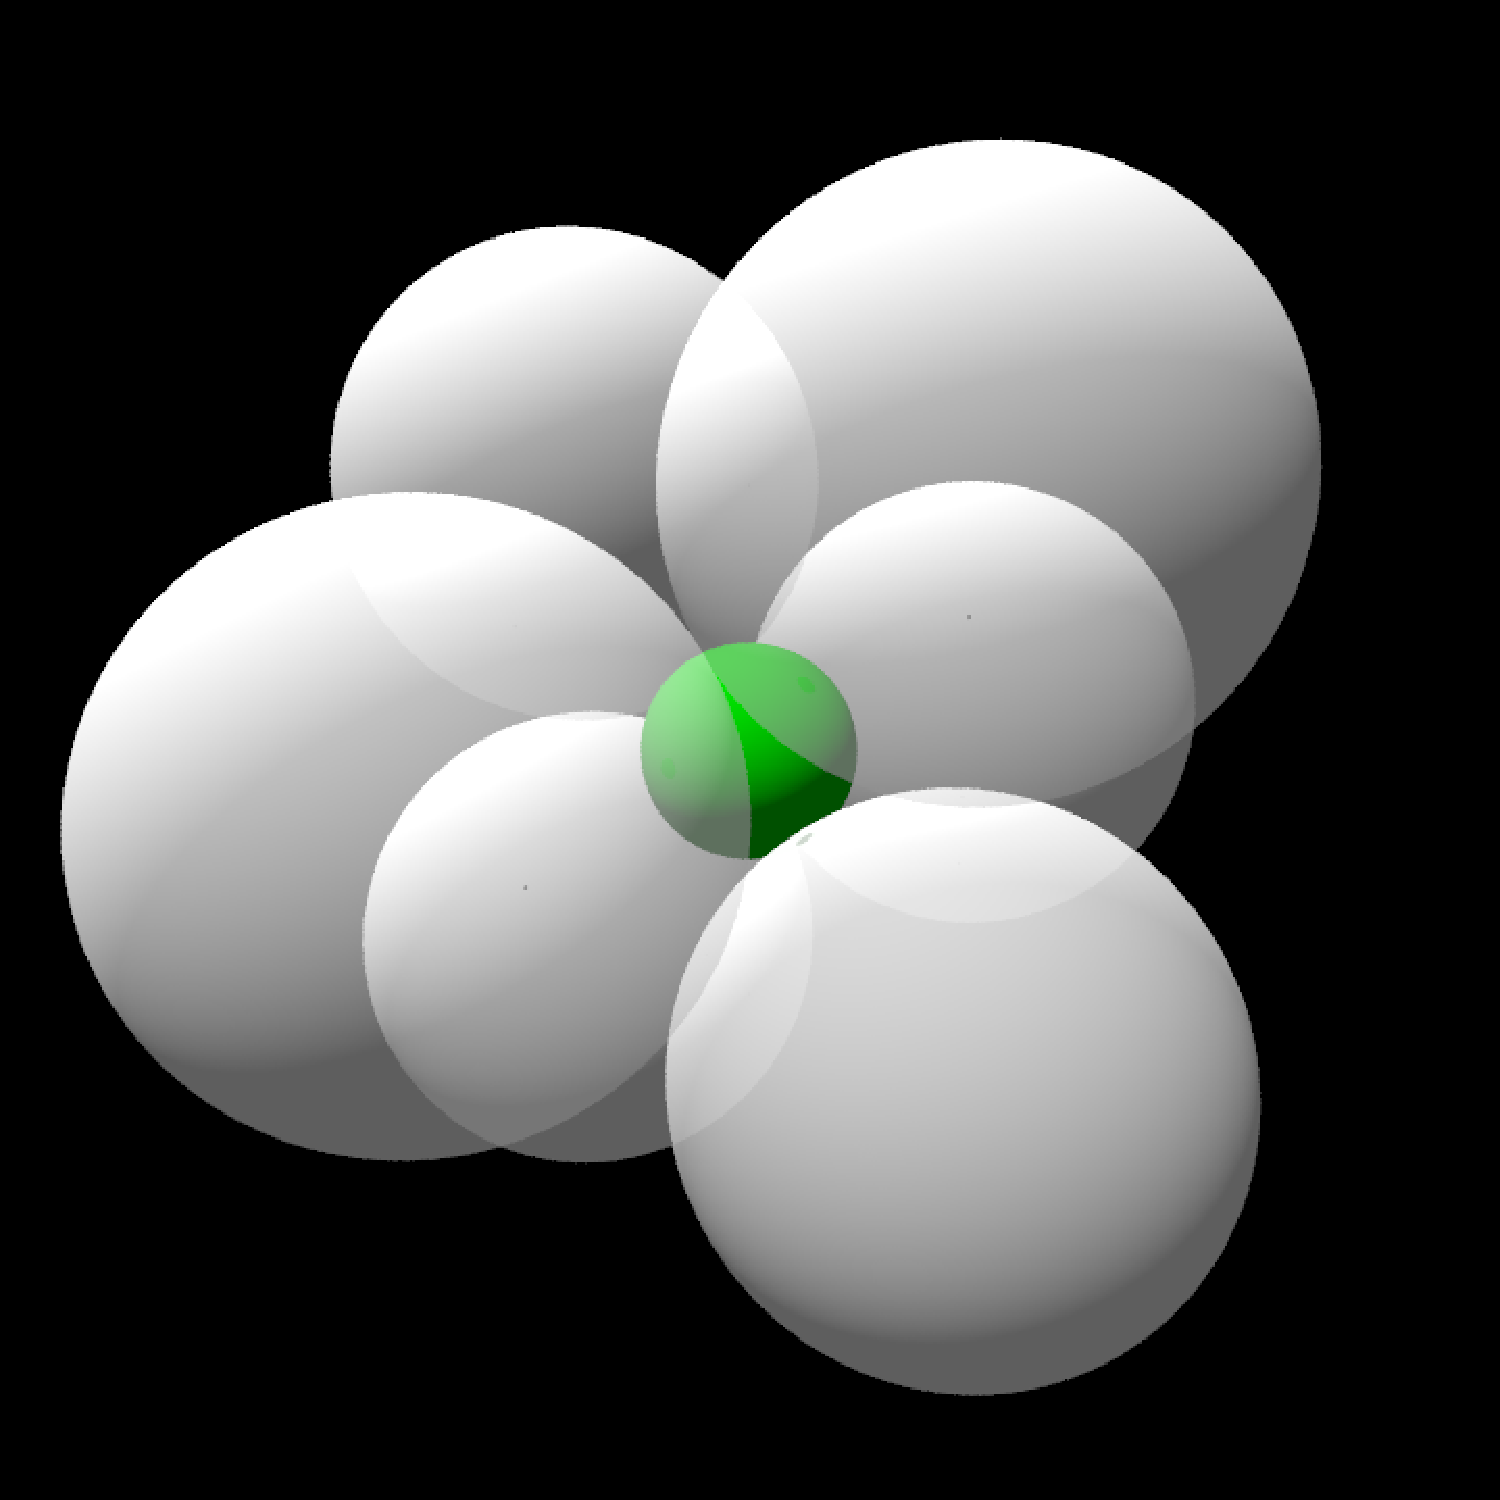
\includegraphics[ height=1.5in, keepaspectratio]{../img/klein/simpleGen.pdf}
   \subcaption{Generator}
   \label{fig:simpleGen3d}
  \end{minipage}
  \begin{minipage}[]{0.49\hsize}
   \center
   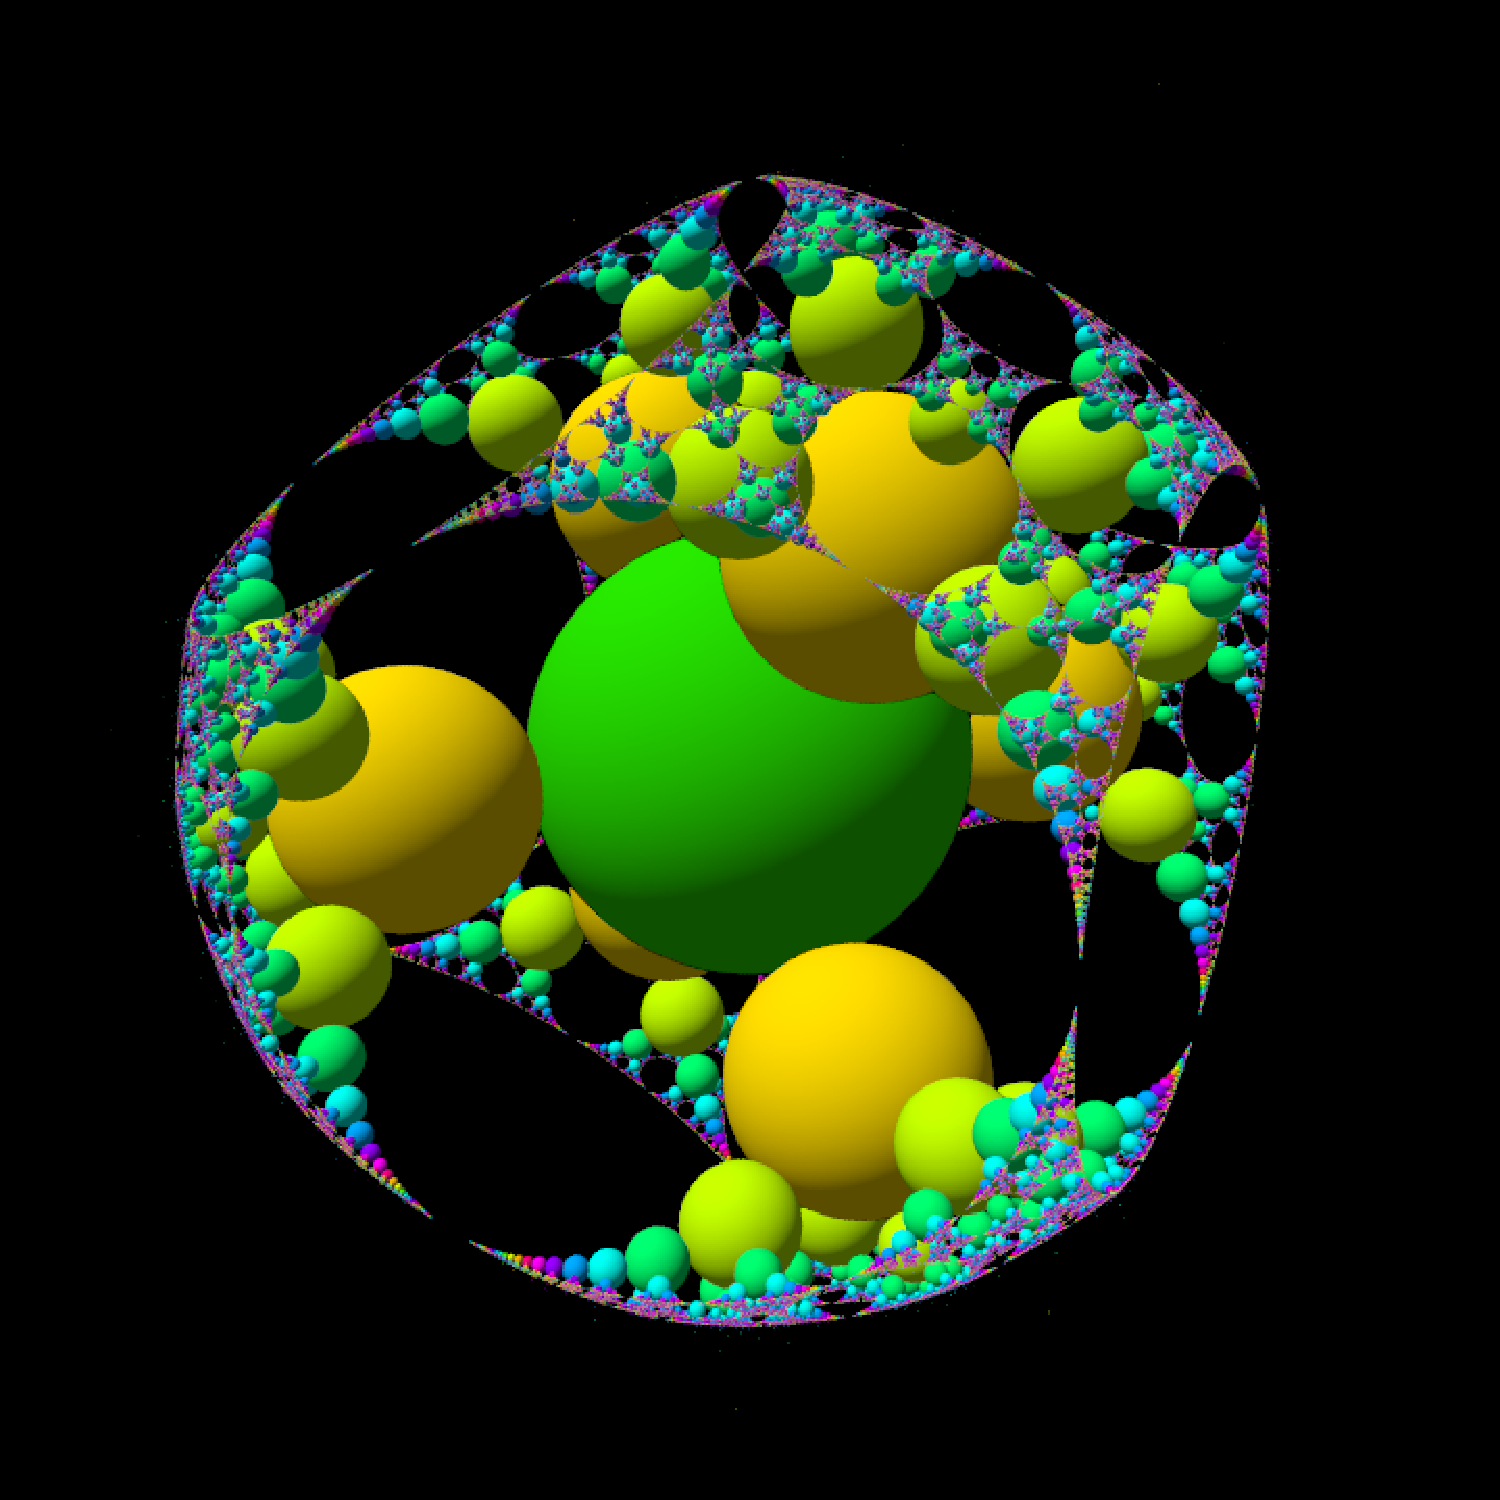
\includegraphics[ height=1.5in, keepaspectratio]{../img/klein/simpleOrbit.pdf}
   \subcaption{Orbit}
   \label{fig:simpleOrb3d}
  \end{minipage}
  \caption{The orbit of the green sphere}
  \label{fig:iis-orb}
 \end{minipage}
 \begin{minipage}[b]{0.5\hsize}
  \center
  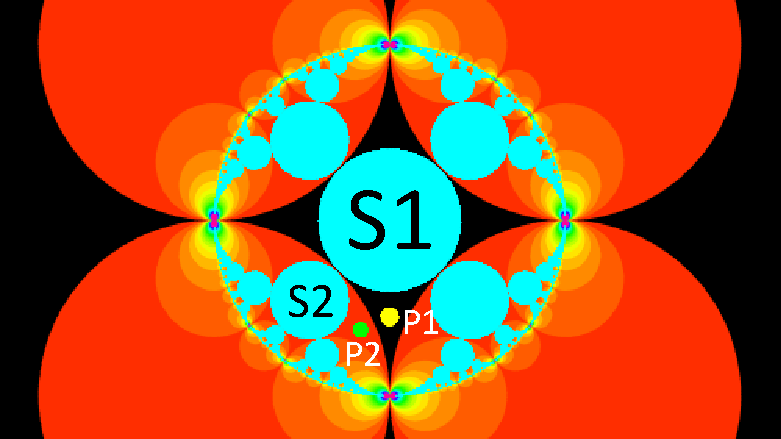
\includegraphics[ height=1.5in, keepaspectratio]{../img/klein/xySlice.pdf}
  \caption{XY-slice image of Figure \ref{fig:iis-orb}}
  \label{fig:xySlice}
 \end{minipage}
\end{figure}

\begin{figure}[htbp]
 \begin{minipage}{0.5\hsize}
  \center
  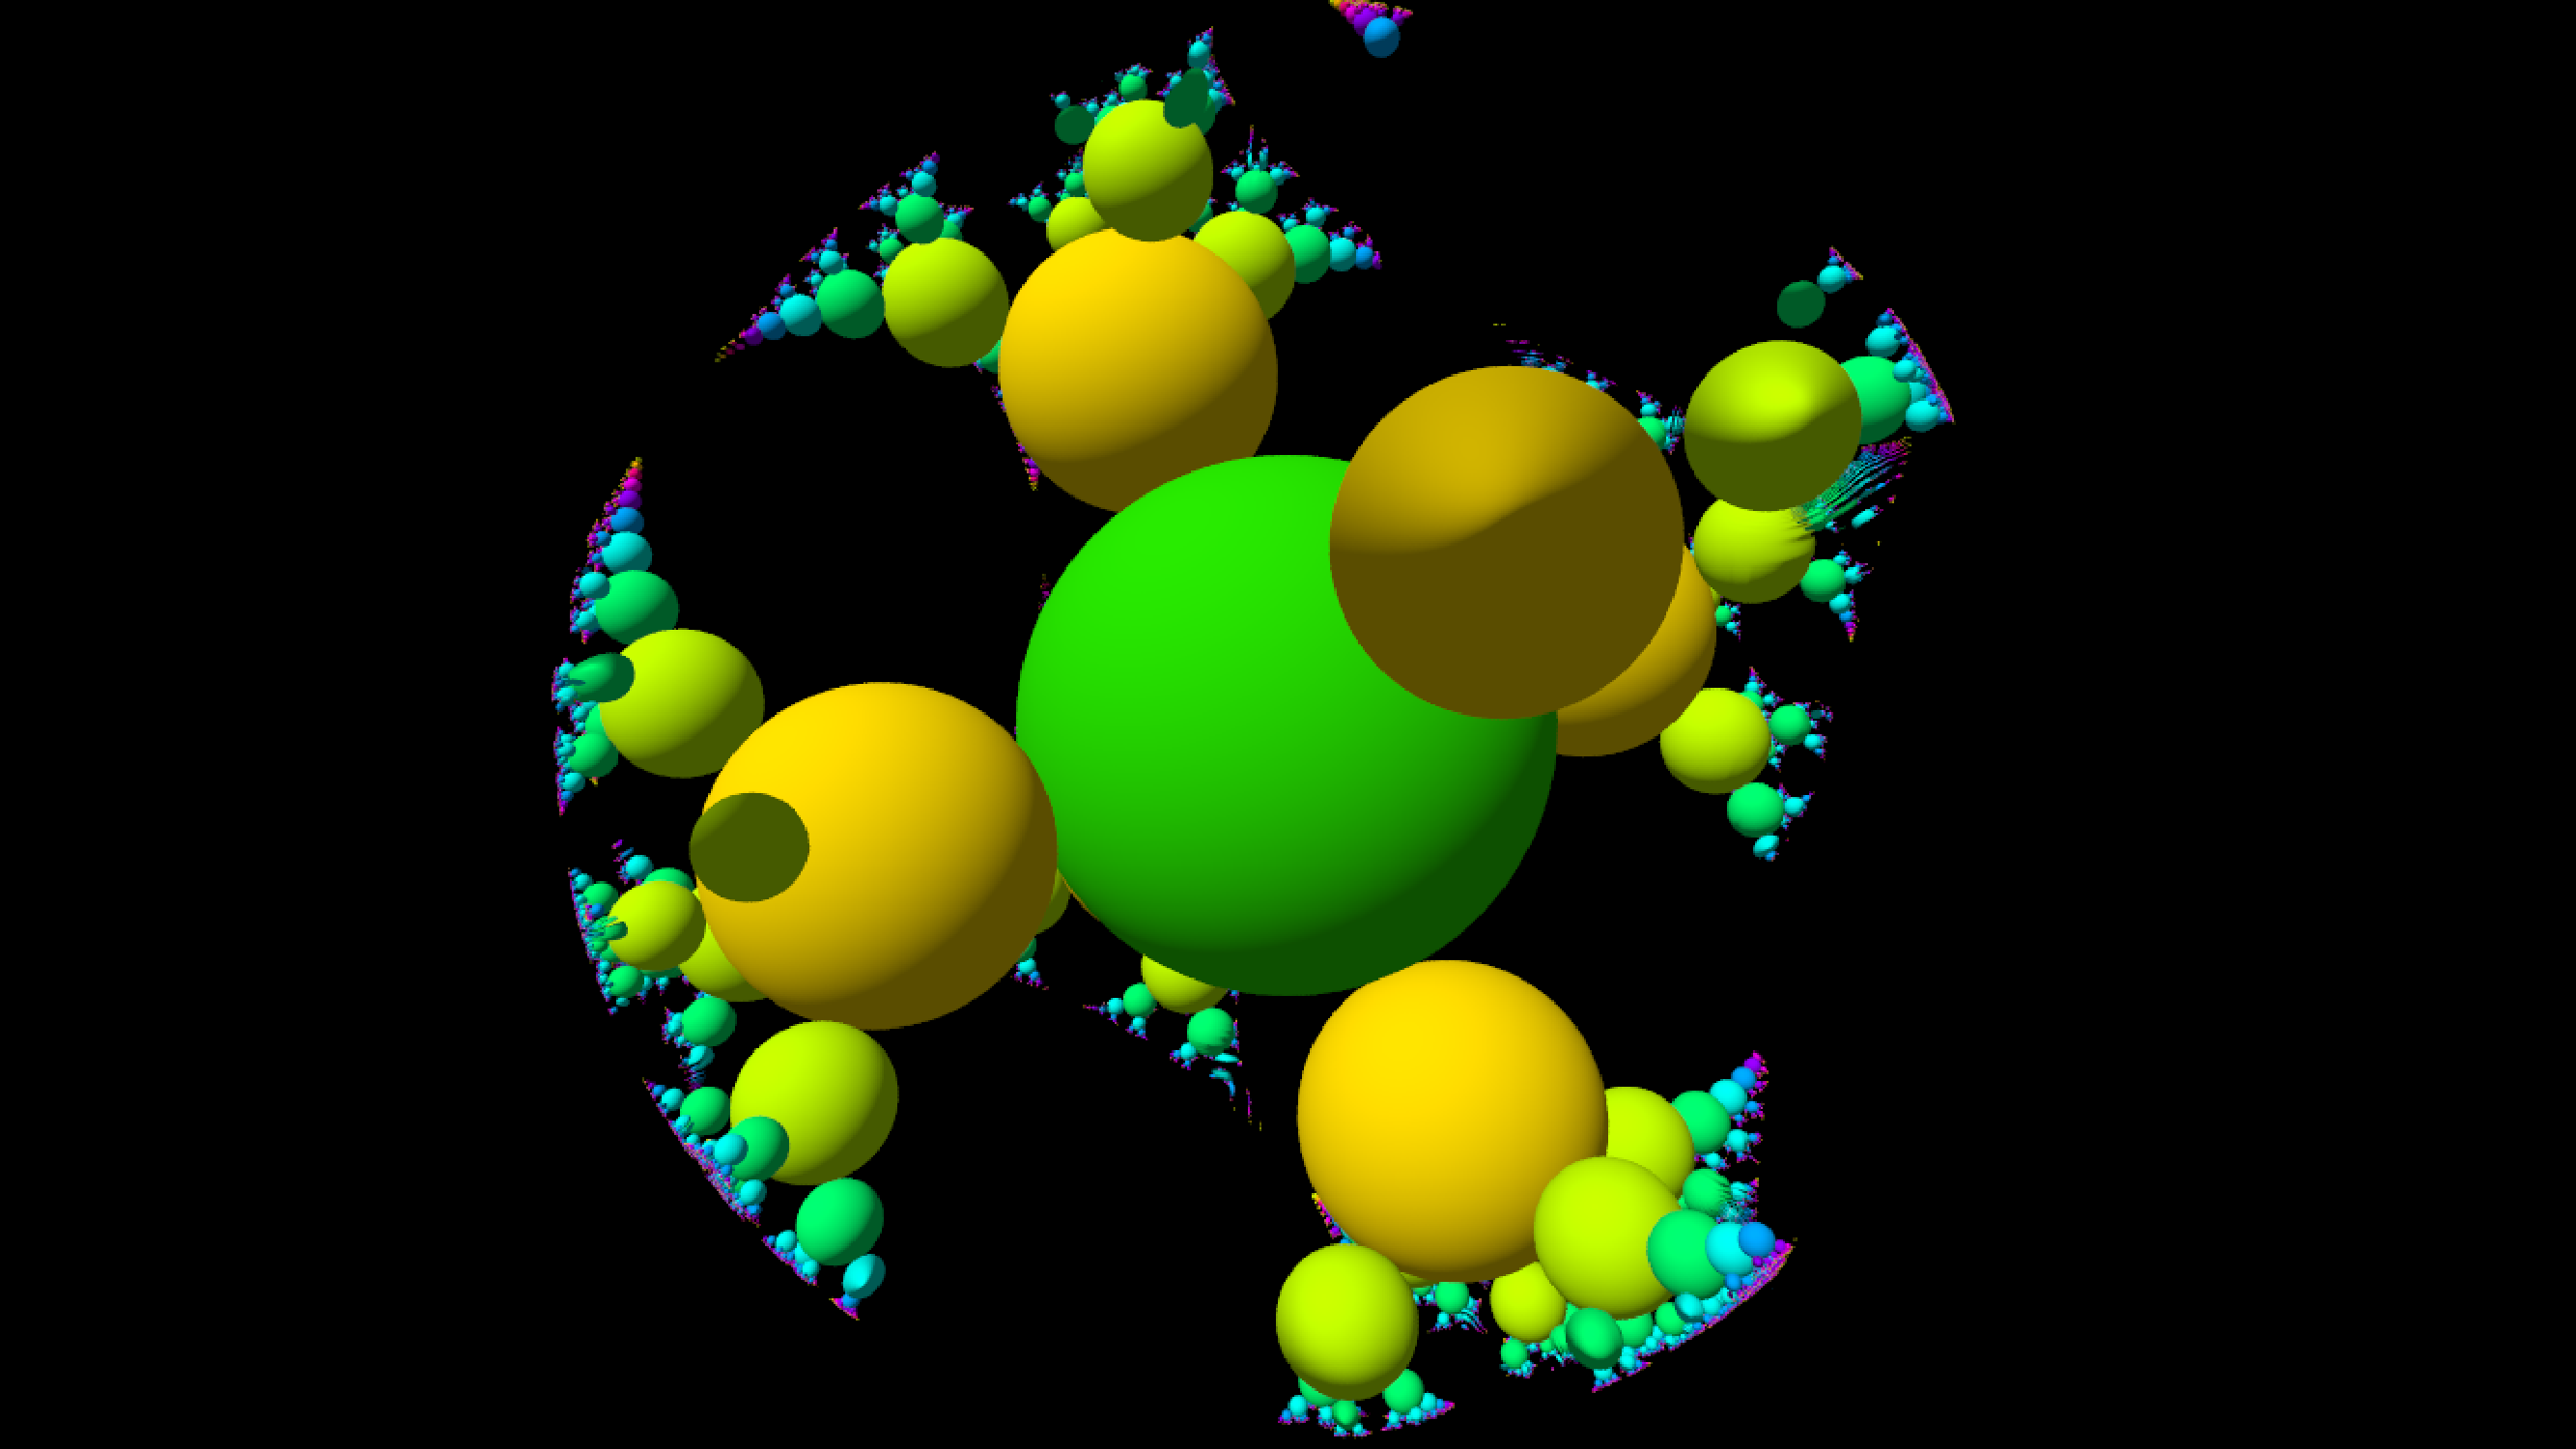
\includegraphics[ height=1.5in, keepaspectratio]{../img/klein/artifact.pdf}
  \caption{The Artifact}
  \label{fig:artifact}
 \end{minipage}
 \begin{minipage}{0.5\hsize}
  \center
  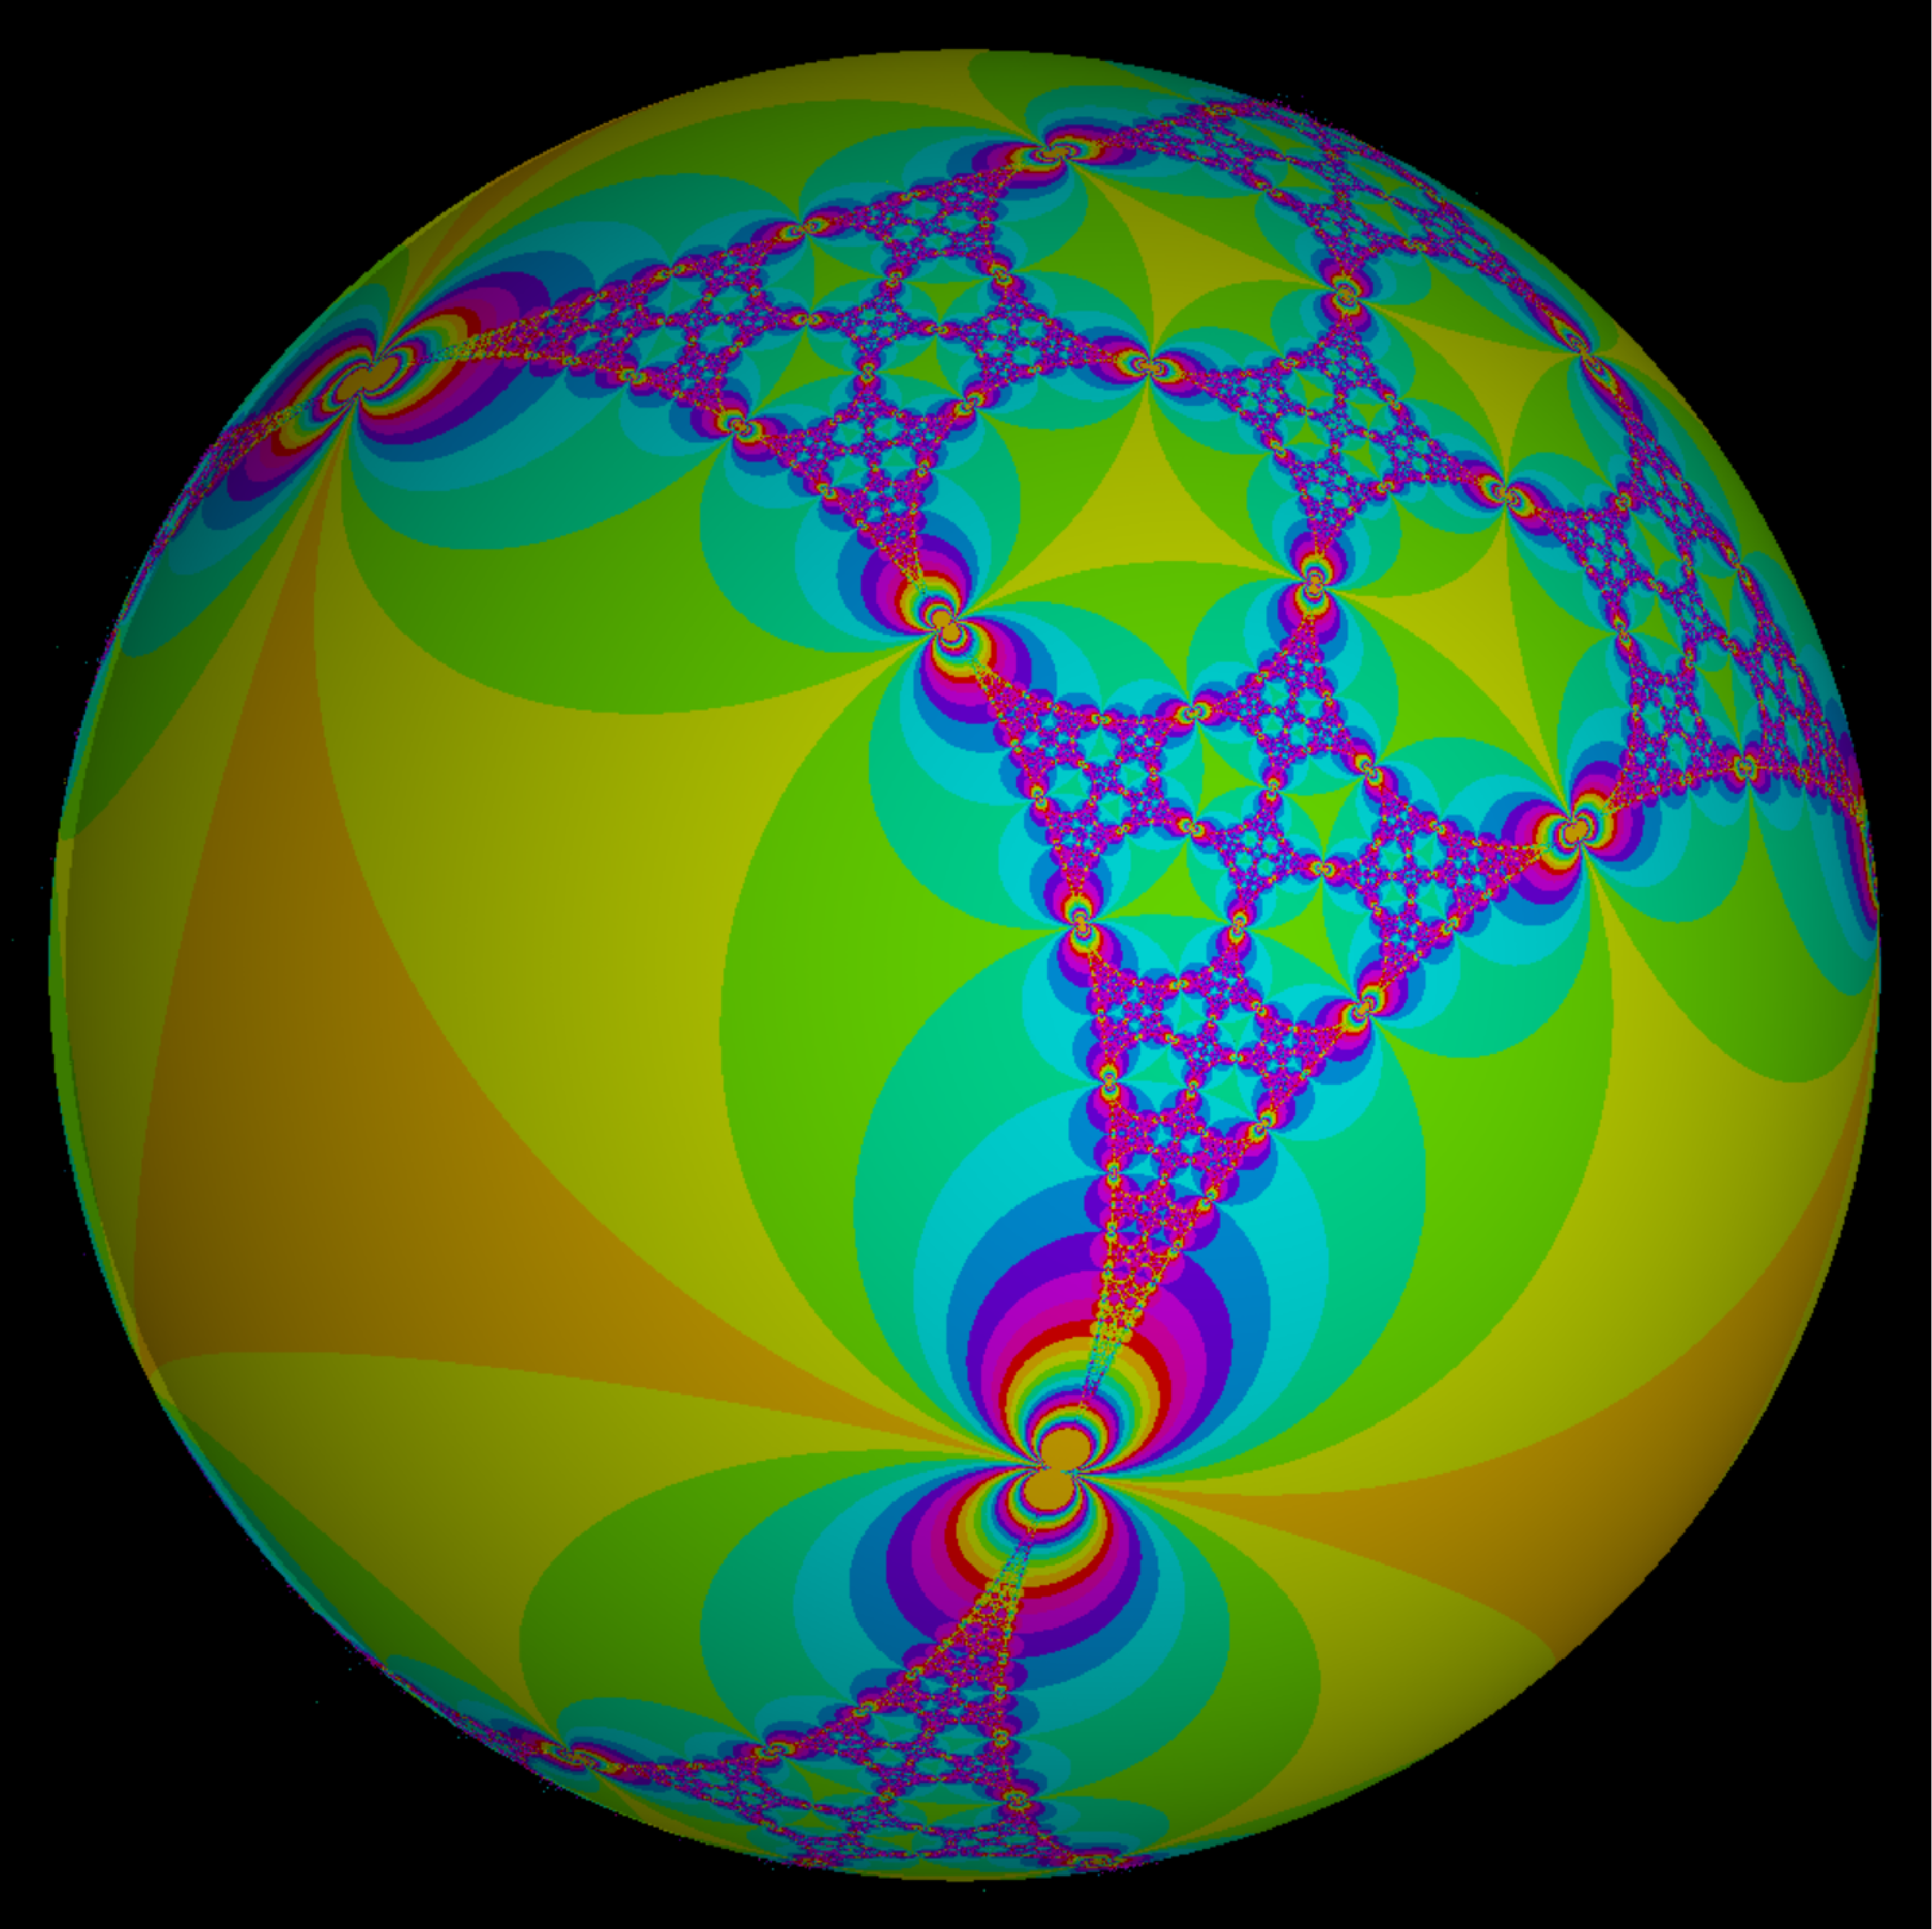
\includegraphics[ height=1.5in, keepaspectratio]{../img/klein/3dLimitSet.pdf}
  \caption{The Limit set on the sphere}
  \label{fig:limitSetOnSphere}
 \end{minipage}
\end{figure}

\begin{figure}[htbp]
 \begin{minipage}{0.5\hsize}
  \center
  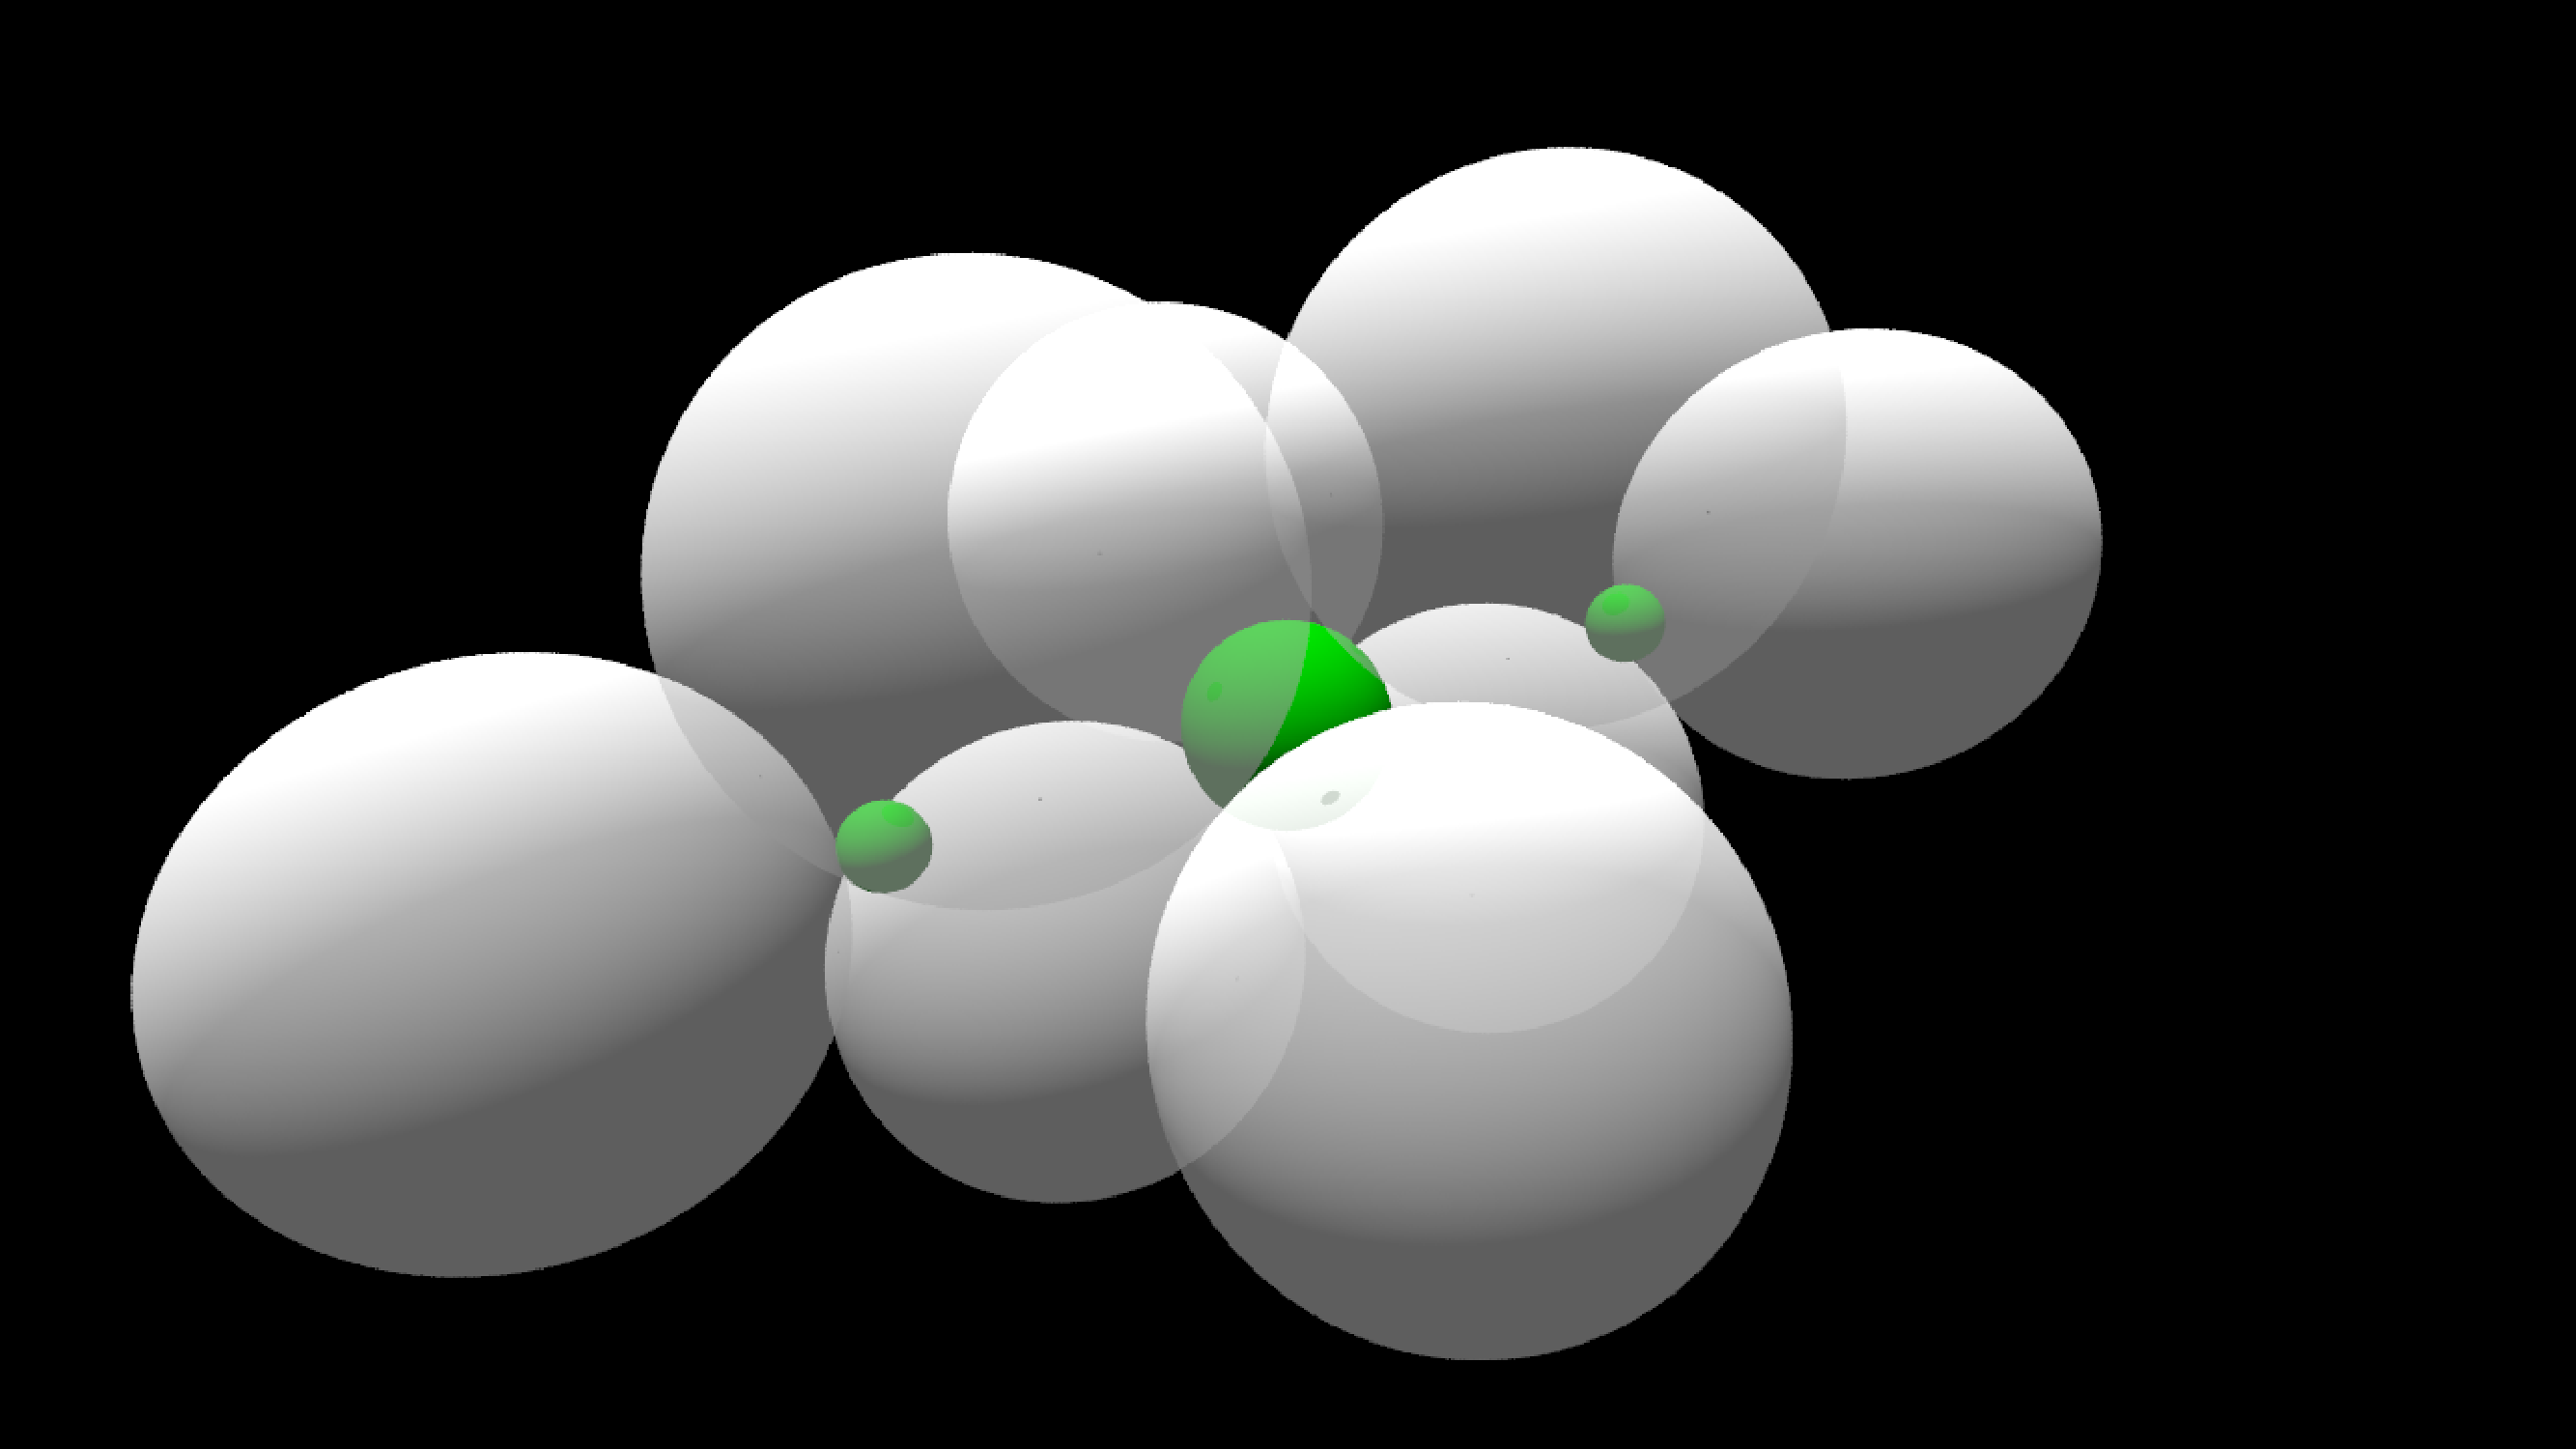
\includegraphics[ height=1.5in, keepaspectratio]{../img/klein/3baseGen.pdf}
  \subcaption{Generator}
  \label{fig:}
 \end{minipage}
 \begin{minipage}{0.5\hsize}
  \center
  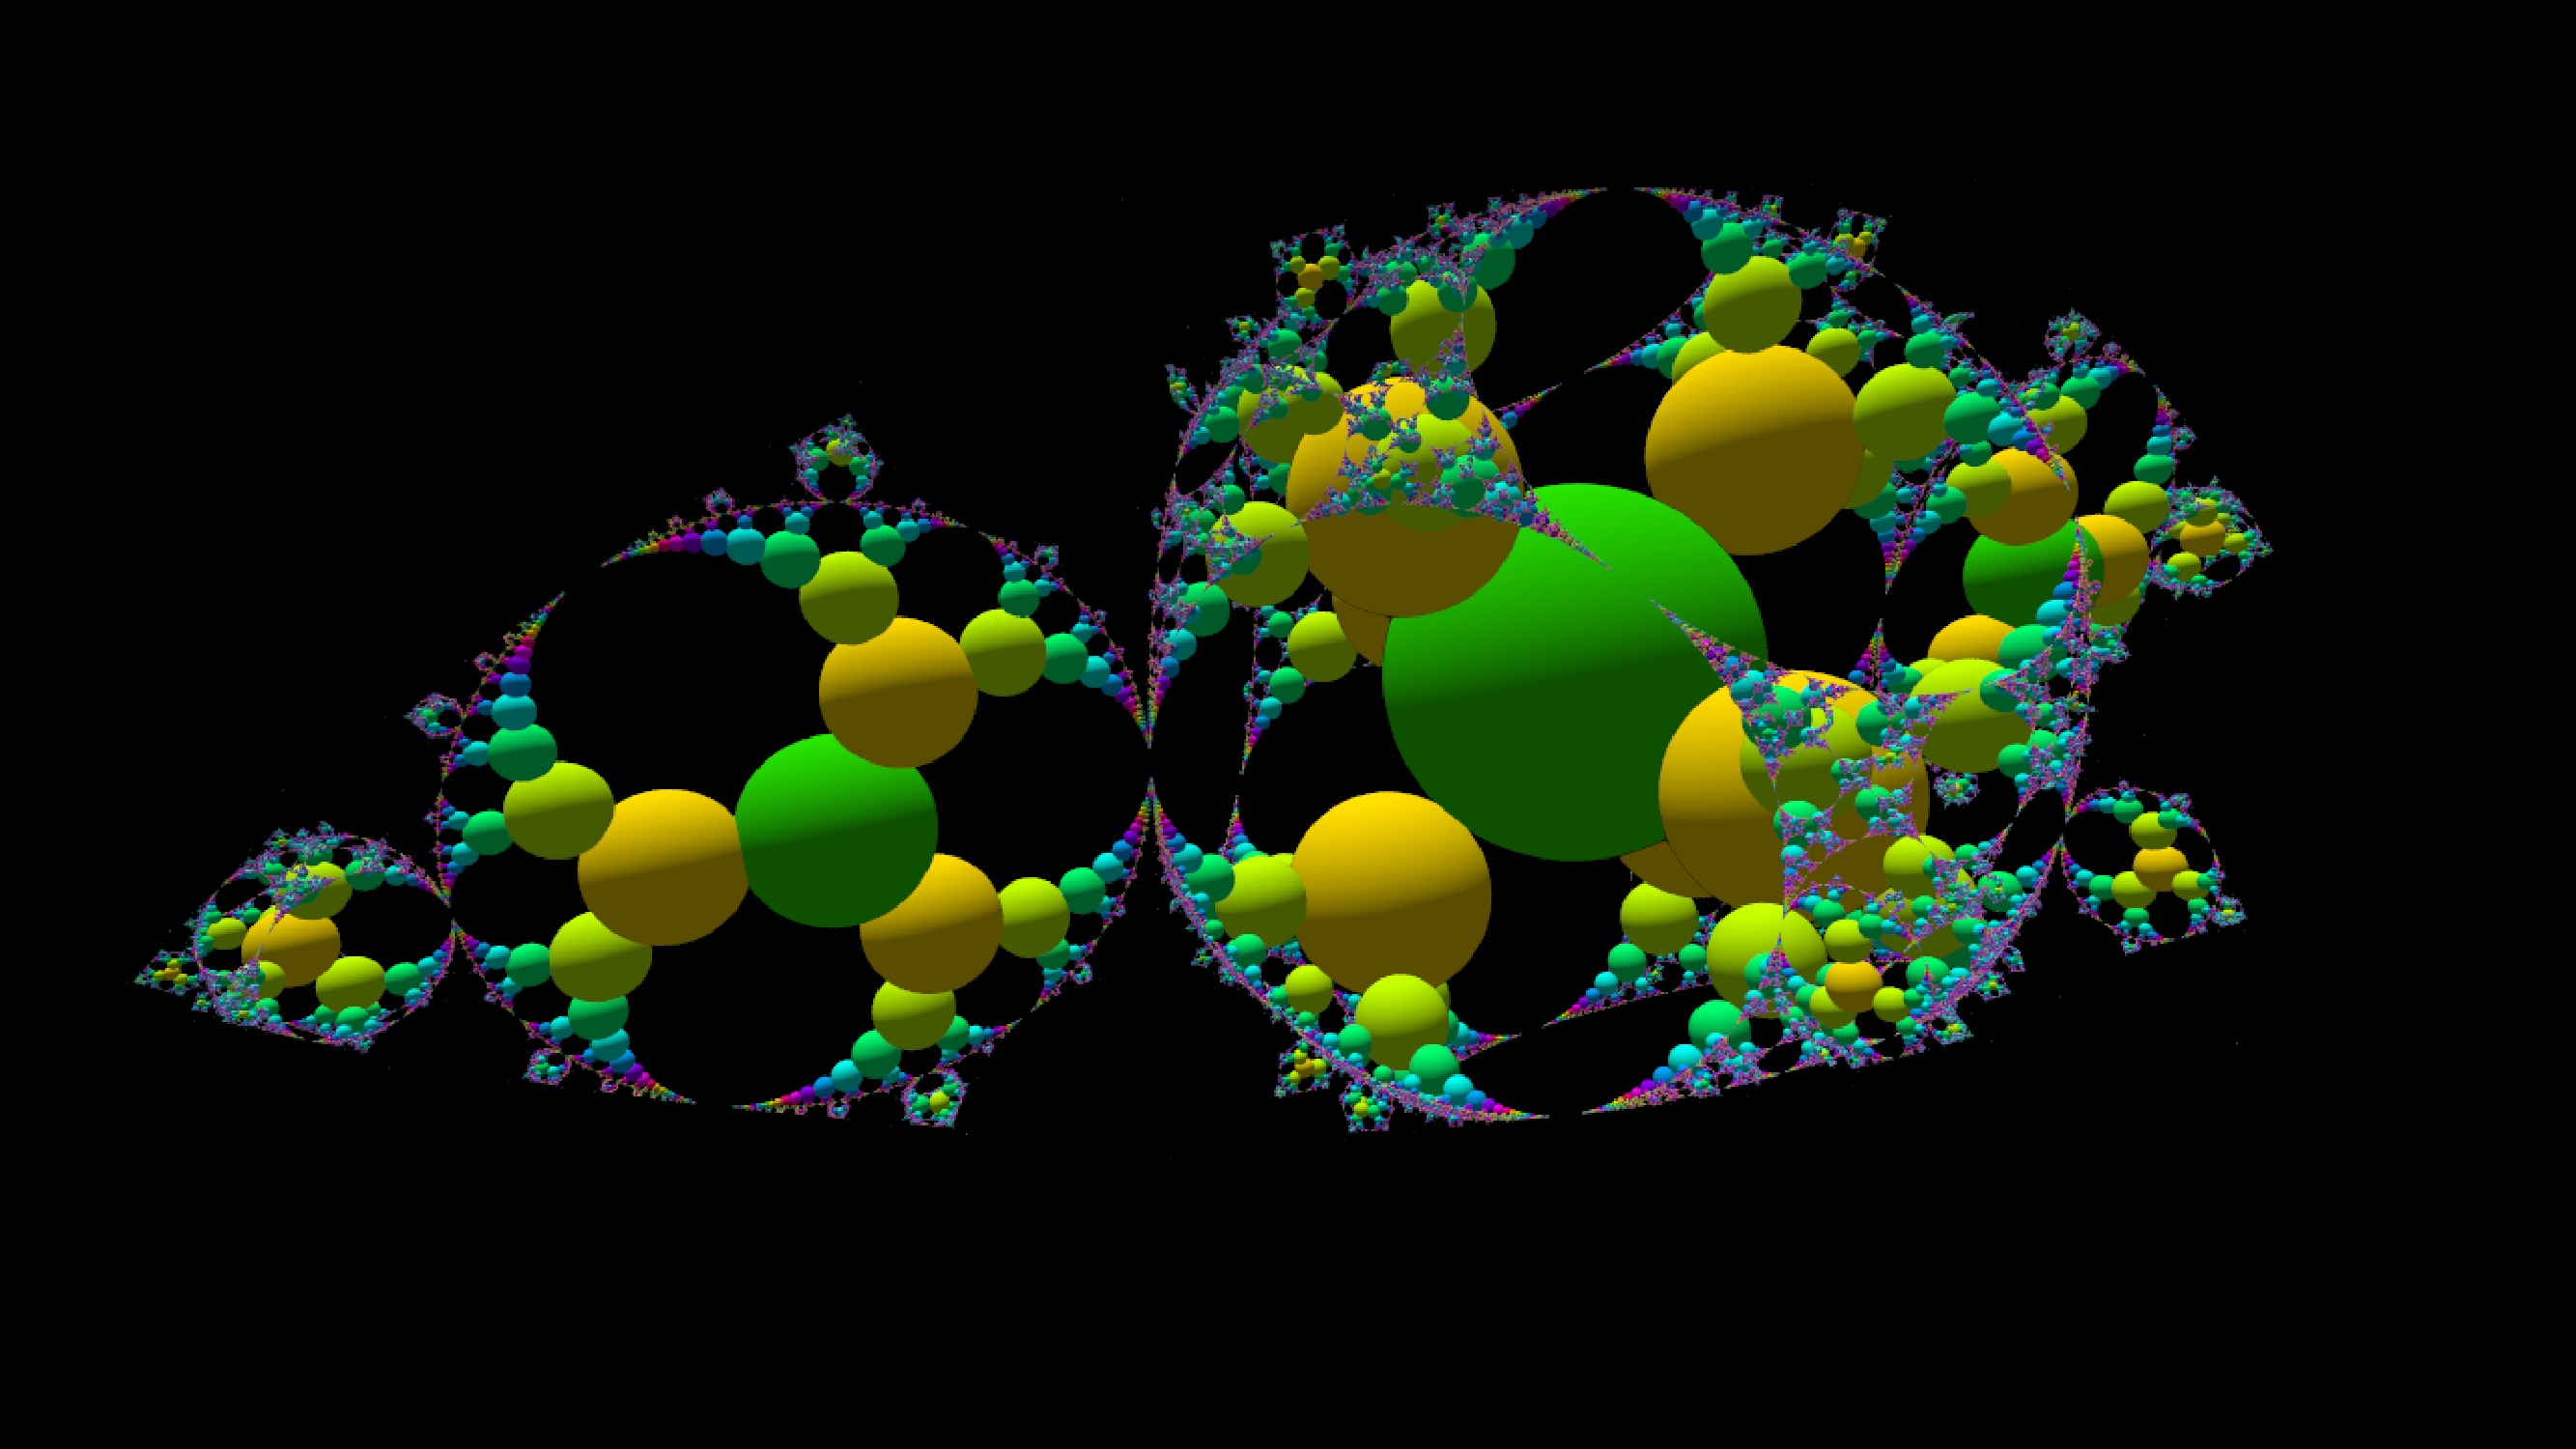
\includegraphics[ height=1.5in, keepaspectratio]{../img/klein/3baseOrb.pdf}
  \subcaption{Orbit}
  \label{fig:}
 \end{minipage}
 \caption{The orbit of 3 base spheres}
 \label{fig:3baseSphere}
\end{figure}

\begin{algorithm}
 \caption{Distance function}
 \label{iis3d}
 \begin{algorithmic}
  \REQUIRE count $= 0$, $d$ = MAX\_DISTANCE, $dr = 1.0$, and coordinates $=$ tipping
  point of the ray
  \FOR{$i=0$ to MAX\_INVERSION}
  \STATE inFundamentalDomain $\leftarrow$ \TRUE
  \FOR{ each Map $G$ in Maps}
  \IF{$G$ is available to coordinates}
  \STATE coordinates $\leftarrow$ $G(\text{coordinates})$
  \STATE $dr \leftarrow dr * $ (Jacobian of $G(\text{coordinates})$)
  \STATE INCREMENT count
  \STATE inFundamentalDomain $\leftarrow$ \FALSE
  \ENDIF
  \ENDFOR
  \IF {isInFundamentalDomain}
  \STATE BREAK for
  \ENDIF
  \ENDFOR
  \FOR{ each BaseSphere $S$ in BaseSpheres}
  \STATE $d \leftarrow$ min($d$, scalingFactor * (distance(coordinates, $S$.center) $-$
  $S$.radius) $/$ (absolute value of $dr$))
  \ENDFOR
  \RETURN $d$
 \end{algorithmic}
\end{algorithm}

\subsection{Geometrical Representation of M\"obius Transformations}

木構造を用いて群を可視化する際には,変換を行列で考えたが,行列表現でメビ
ウス変換を操作することは直観が得にくい.
さらに,四次元クライン群を構成する三次元空間に作用するメビウス変換は, 2×2
四元数行列で表現することができるが,さらにパラメータ数が増大する.
このことは,四次元クライン群の研究を難しくしている.
そこで筆者はすべてのメビウス変換を円や球の反転で構成することを考えた.
円や球を用いることで,生成元と可視化される図形の間の関係性が理解しやすく,
幾何学的な直観を得ることができる.
それに加え,IISを用いることで複雑な生成元をもつ群もリアルタイムに可視化
することができる.
このことは,研究者や学習者だけでなく,フラクタルアーティストにも有益なも
のとなるだろう.
また,筆者は円や球の反転で構成される群をインタラクティブに構成するソフト
ウェア, {\it Schottky Link} \footnote{Schottky Link:
\url{https://schottky.jp}}を開発している.

\subsubsection{2D Generators}

\noindent\textbf{Simple Inversion}
先に述べたように, 円に関する反転は複素平面の向きを変えるので, メビウス変
換ではない.
ふたつの反転円がペアとなってはじめてメビウス変換となる.
しかし, ここでは簡単のためにメビウス変換の元として扱う.

\noindent\textbf{Inversion of a Circle with Infinite Radius}
無限の半径をもつ円に関する反転は直線に関する反転で表される.
図では右側の反転円が左側の半径無限の円の内側に反転で移されていることがわ
かる.

\noindent\textbf{Rotation}
二つの交差する直線の反転の組み合わせは回転を表わす. 回転角は二直線のなす
角の二倍である. 図では90度回転を示した. また, 軌道となる円同士がお互いに
重なりあわないようにするためには, 回転角は有理角である必要がある.

\noindent\textbf{Composition of Two Circles}
二つの同心円をもちいることで, 双曲型変換である単純な拡縮を表わすことがで
きる.
図をみよ.
赤い円を$C1$,緑の円を$C2$, そして青い円を$C1'$とよぶ.
$C1'$は$C1$を$C2$による反転で移した像である.
図では, 白い縁をもつ二つの円の軌道を描いている.
固定点は円の中心と無限遠点である.
我々は写像$G$を以下のように構成する.
ここで接頭辞$I$は反転を表わす.
例えば, $I_{C1}$は$C1$による反転を表わす.
\begin{align*}
 G =
  \begin{cases}
   I_{C2} \circ I_{C1} & (\text{The point is inside of } C1) \\
   I_{C1} \circ I_{C2} & (\text{The point is outside of }C1')
  \end{cases}
\end{align*}
我々は$G$を繰り返し用いることで点を基本領域へと移動させることができる.
この種類の生成元の基本領域は青と緑の領域である.
完全な円の軌道をIISを用いて描くには, ショットキー円をこの領域内に配置す
る必要がある.

次に, $C1$を少し動かすと, 図のような軌道が得られる.
有限の固定点は動くが, 内側の円$C1$の内部に留まり, 無限遠点の固定点は有限
の点に移る.
二つの円が交差しない限り, これも双曲型変換である.
$C1$と$C2$が接触する時, 図のように固定点はその交点で重なりあい, 放物型変
換となる.

\noindent\textbf{Loxodromic}
上記の生成元の軌道は単純な拡縮と共役であった.
我々はその軌道に二つの反転を加えることで軌道を捻ることができる.
図では$C1$の中心を$C2$通る白い直線$L$と黄色の円$C3$, そして水色の点$P$が
描かれている.
$P$は制御点であり, $C3$は$P$とその$C1$と$C2$による反転の像である$P'$と
$P''$の三点から定義される.
$L$と$C3$の組み合わせは回転を表す.
写像$G$は以下のようになる.
\begin{align*}
G =
\begin{cases}
 (I_{C2} \circ I_{C1}) \circ (I_{C3} \circ I_L) & (\text{The point is inside of } C1) \\
 (I_L \circ I_{C3}) \circ (I_{C1} \circ I_{C2}) & (\text{The point is outside of }C1')
\end{cases}
\end{align*}
また, 二つの固定点からこの種類の生成元を得ることもできる.

\subsubsection{3D Generators}
ほとんどの三次元の生成元は二次元の生成元から自然に導くことができる.

\noindent\textbf{Simple Inversion.}
二次元の場合と同様に球の反転単体はメビウス変換ではなく, 二つの球のペアに
よる反転がメビウス変換である.
しかし, ここではこれもメビウス変換として扱う.

\noindent\textbf{Inversion of a Sphere with Infinite Radius}
半径が無限大の球による反転は平面による反転と表すことができる.
図では青い板が半径が無限の球を表現している.
右側の軌道はこの板によって左側へと移されている.

\noindent\textbf{Rotation}
二次元の場合と同様にして, 回転は互いに交わる二枚の平面の反転により表され
る.
回転軸は二枚の平面の交線である.
図では180度の回転を示した.

\noindent\textbf{Parallel Translation}
二つの平行な平面のペアは平面の法線方向への平行移動を表わす.
図はこの生成元と軌道を描いた.
これは, 放物型変換である.

\noindent\textbf{Compound Parabolic}
更に, 三次元では, 軌道に捻りを加えることができる.
図では軌道に平行移動の元が適用されるたびに回転していることがわかる.
これは\emph{複合放物型変換}(\textit{Compound Parabolic})とよばれる.

\noindent\textbf{Composition of Two Spheres}

二次元の場合と同様に二つの球の反転を組み合わせる.
図に示される赤い球を$S1$, 黄緑の球を$S2$,青い球を$S1'$とよぶ.
写像$G$は二次元と同様に以下のようになる.
\begin{align*}
G =
\begin{cases}
 I_{S2} \circ I_{S1} & (\text{The point is inside of } S1) \\
 I_{S1} \circ I_{S2} & (\text{The point is outside of }S1')
\end{cases}
\end{align*}
$S1$と$S2$に接触がない場合この生成元は斜航型変換である.
軌道は図に示した.
$S1$と$S2$が一点で接触し時, 放物型変換となる.
その接点が固定点となる.
図をみよ.
球の軌道は固定点ので接触していることがわかる.

\noindent\textbf{Compound Loxodromic}
最後に, $S1$と$S2$に垂直な二つの球を追加する.
図に示される桃色の球を$S3$, 黄色の球を$S4$と呼ぶ.
また, 3つの制御点を$P$,$Q1$,$Q2$が存在する.
$S3$と$S4$の反転の組み合わせは回転を表す.
球は4つの点により決定される.
$P'$と$P''$を$P$の$S1$と$S2$の反転による像とする.
$G$は以下のようになる.
\begin{align*}
S3 = Sphere(P, P', P'', Q1) \quad
S4 = Sphere(P, P', P'', Q2) \\
G =
\begin{cases}
 (I_{S4} \circ I_{S3}) \circ (I_{S1} \circ I_{S2}) & (\text{The point is inside of } S1) \\
 (I_{S2} \circ I_{S1}) \circ (I_{S3} \circ I_{S4}) & (\text{The point is outside of }S1')\\
\end{cases}
\end{align*}
図では, 二次元における斜航型変換のような捻じれた軌道をみることができる.
この生成元を\emph{複合斜航型変換}(Compound Loxodromic)とよぶ.

\subsection{Optimization}

いくつかの反転で構成された写像は適切な共役をとることによって, 最適化する
ことができる.
この節では, 二次元の生成元における
最適化された写像は点を基本領域に一度の操作で移動させる.

\noindent\textbf{Parallel Translation.}
図と同様の平行な二直線の組を考える.
繰り返し反転を適用する代わりに, 剰余を用いて点を写像することができる.
まず始めに, 与えられた点を今回の共役変換である平行移動と回転を用いて, 平
行な二直線が, X軸に垂直に, 片方の直線がY軸に沿うようにする.
共役変換で移された直線は図に示した.
$w$を二直線の距離, $i$を図における帯の指数, $P$を写像に与えられた点,
$P'$を写像によって移された点, $d$と$d'$をY軸からの距離とする.
我々は$d$を$w$で割ることにより, 剰余$d'$と商$i$を得る.
最後に$d'$を用いて$P'$を計算し, これを共役変換で座標に戻す.

\noindent\textbf{Parabolic.}
次に図のような放物型変換を考える.
まず共役変換$T$をこの変換の固定点を中心とする円の反転とする.
$T$を$C1,C2,C1'$に対して適用すると, 固定点は無限遠点に移るので, 三本の平行な直
線を得ることができる.
これらの直線を$TC1, TC2, TC1'$とよぶ.
図ではこれらの直線が示されている.
赤の直線$TC1$と青の直線$TC1'$が平行移動を表す.
写像の過程は以下のようになる.
まず, $T$を与えられた点$P$に適用し, $T(P)$を得る.
そして, $T(P)$を平行移動と同様にして移し, $P'$を得る.
最後にもう一度$T(= T^{-1})$を$P'$に適用する.

\noindent\textbf{Loxodromic}
最後に図のような双曲型変換を考える.
共役変換$T$を片方の固定点を中心にもつ円に関する反転とする.
$T$を$C1, C2, C1'$に適用した像を$TC1, TC2, TC1'$とよび, これらは, もう一
方の固定点の反転した像を中心にもつ同心円となる.
これは実数倍を表す.
図において, $P$を写像に与えられた点, $P'$を写像された点, $r$と$r'$を
$TC1$と$TC1'$の半径, $d$と$d'$を$TC1$からの距離, $k$を倍数, $q$を
$exponential ciefficient$,  $i$を円列の指数とする.
これらは以下のように計算される.
 \begin{math}
  k = \frac{r'}{r},
  q = \log_{k} \frac{d}{r},
  d' = r \cdot k^{fracionalPart(q)},
  i = floor(q).
 \end{math}
我々は$d'$を用いて$P'$を計算することができる.

また, 図のような双曲型変換であるとき, $T$を$L$と$C3$にも適用し, その像を
$TL$と$TC3$とよぶ.
図は複素数によるスケーリングを表している.
白い直線$TL$と黄色の直線$TC3$は同心円の中心で交わっている.
$P'$を得た後で回転を与えて$P''$を得る.
$TL$と$TC3$のなす角を$\theta$, 回転角を$\varphi$とすると, $\varphi$は
$\varphi = 2 \theta i$で計算することができる.

まず, $T$を与えられた点$P$に適用し, $T(P)$を得る.
そして, $d'$を用いて$P'$を計算する.
もしも交差する直線があれば, $P'$を$\varphi$回転させ, $P''$を得る.
最後にもう一度$T$を$P'$もしくは$P''$に適用する.

\subsection{Other Topics}

この節では, その他のレンダリング手法とクライン群の研究の中でも興味深い図像を見ることができる先行研究を紹介する.

\subsubsection{Other Rendering Methods}
Aaron MontagはIterated Inversion Systemを拡張したHyperbolic Iterated Function Systemによって極限集合を描画することに成功した\cite{hyperbolicIFS}.固定点付近では図に乱れが出るものの,おおむね描画できる.実装はここ\footnote{Kleinian Groups WebGL: \url{https://www-m10.ma.tum.de/bin/view/Lehrstuhl/AaronMontagKleinian}}でみることができる.

また,Jos Ley, Knighty両氏はマスキット群におけるEscape-timeアルゴリズム
とDistance Estimationを開発した
\footnote{An escape time algorithm for Kleinian group limit set:\\ \quad
\quad \url{http://www.fractalforums.com/3d-fractal-generation/an-escape-tim-algorithm-for-kleinian-group-limit-sets/}}.
 二次元の極限集合だけでなく,三次元の図像も高速に描画することができる.
荒木・糸\cite{maskit}と同様の設定で, 一方に平行移動を含む2つの放物型変換による群を考えている.
詳細なアルゴリズムに関しては, Jos Ley氏がまとめている\footnote{Mathematical Imagery, An escape-time algorithm for a family of Kleinian groups: \url{http://www.josleys.com/article_show.php?id=221}}.

\subsubsection{Quasi Fuchsian 3-Dimensional Fractals}

Quasi Fuchsian 3-Dimensional Fractalsは阿原・荒木による擬フックス群を三次元に拡張した4次元クライン群である\cite{sphairahedra}\cite{sphairahedraJa}.
前述のフラクタルコミュニティに大きな影響を与えたと言われている.

図\ref{fig:schottky}において, 中央の円盤に囲まれた黒い領域を\emph{円辺形}と呼ぶ.
擬フックス群は円辺形を囲む円盤から生成元を得ることができる.
そこで円辺形を三次元に拡張した\emph{球面体}を用いることで三次元の擬フックス群の形状を求めることができる.
図\ref{fig:sphairahedra}は6つの球に囲まれた球面体のひとつである.
三角柱の面は3つの半径無限大の球に囲まれていると考える.
この球面体をそれを囲む球の反転で移していくことで図\ref{fig:quasiFuchsian}のような形状を得る.

著者によってYouTubeに投稿された動画\footnote{Quasi-fuchsian fractals: \url{https://www.youtube.com/watch?v=3lcO9zRCv-4}}ではこのフラクタルの構成過程をみることができる.
数学的な事項については2016年に蔭山氏がまとめている\cite{kageyama}.
荒木はこのフラクタル図形の物質化についてもまとめている\cite{materializing}.
また,Distance EstimationのアルゴリズムがKnightyにより開発された
\footnote{Another 3D Kleinian:
 \url{http://www.fractalforums.com/ifs-iterated-function-systems/another-3d-kleinian/}}.

\begin{figure}[htbp]
 \begin{minipage}{0.49\hsize}
  \begin{center}
   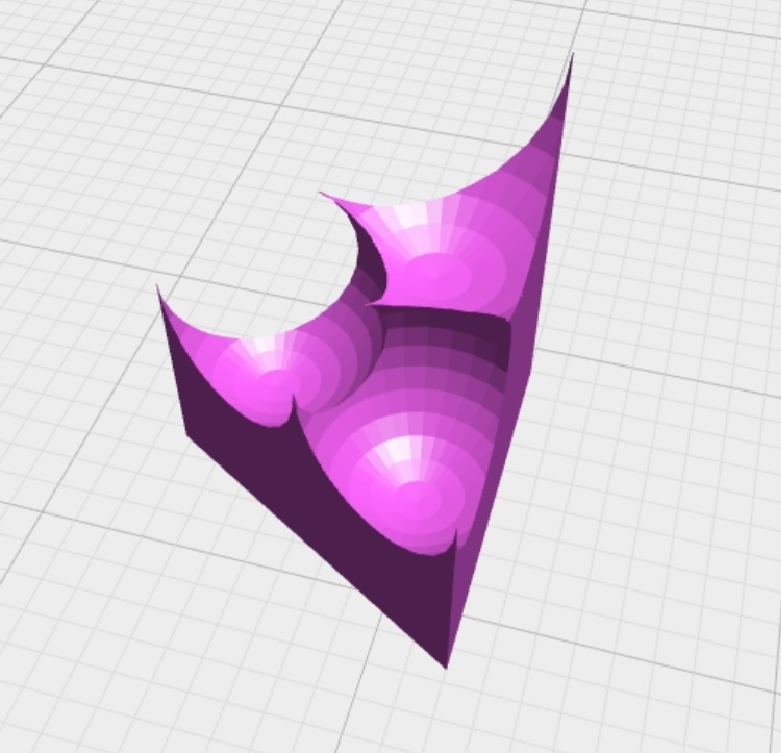
\includegraphics[width=3in, height=3in, keepaspectratio]{../img/klein/sphairahedra.pdf}
   \caption{Sphairahedra}
   \label{fig:sphairahedra}
  \end{center}
 \end{minipage}
 \begin{minipage}{0.49\hsize}
  \begin{center}
   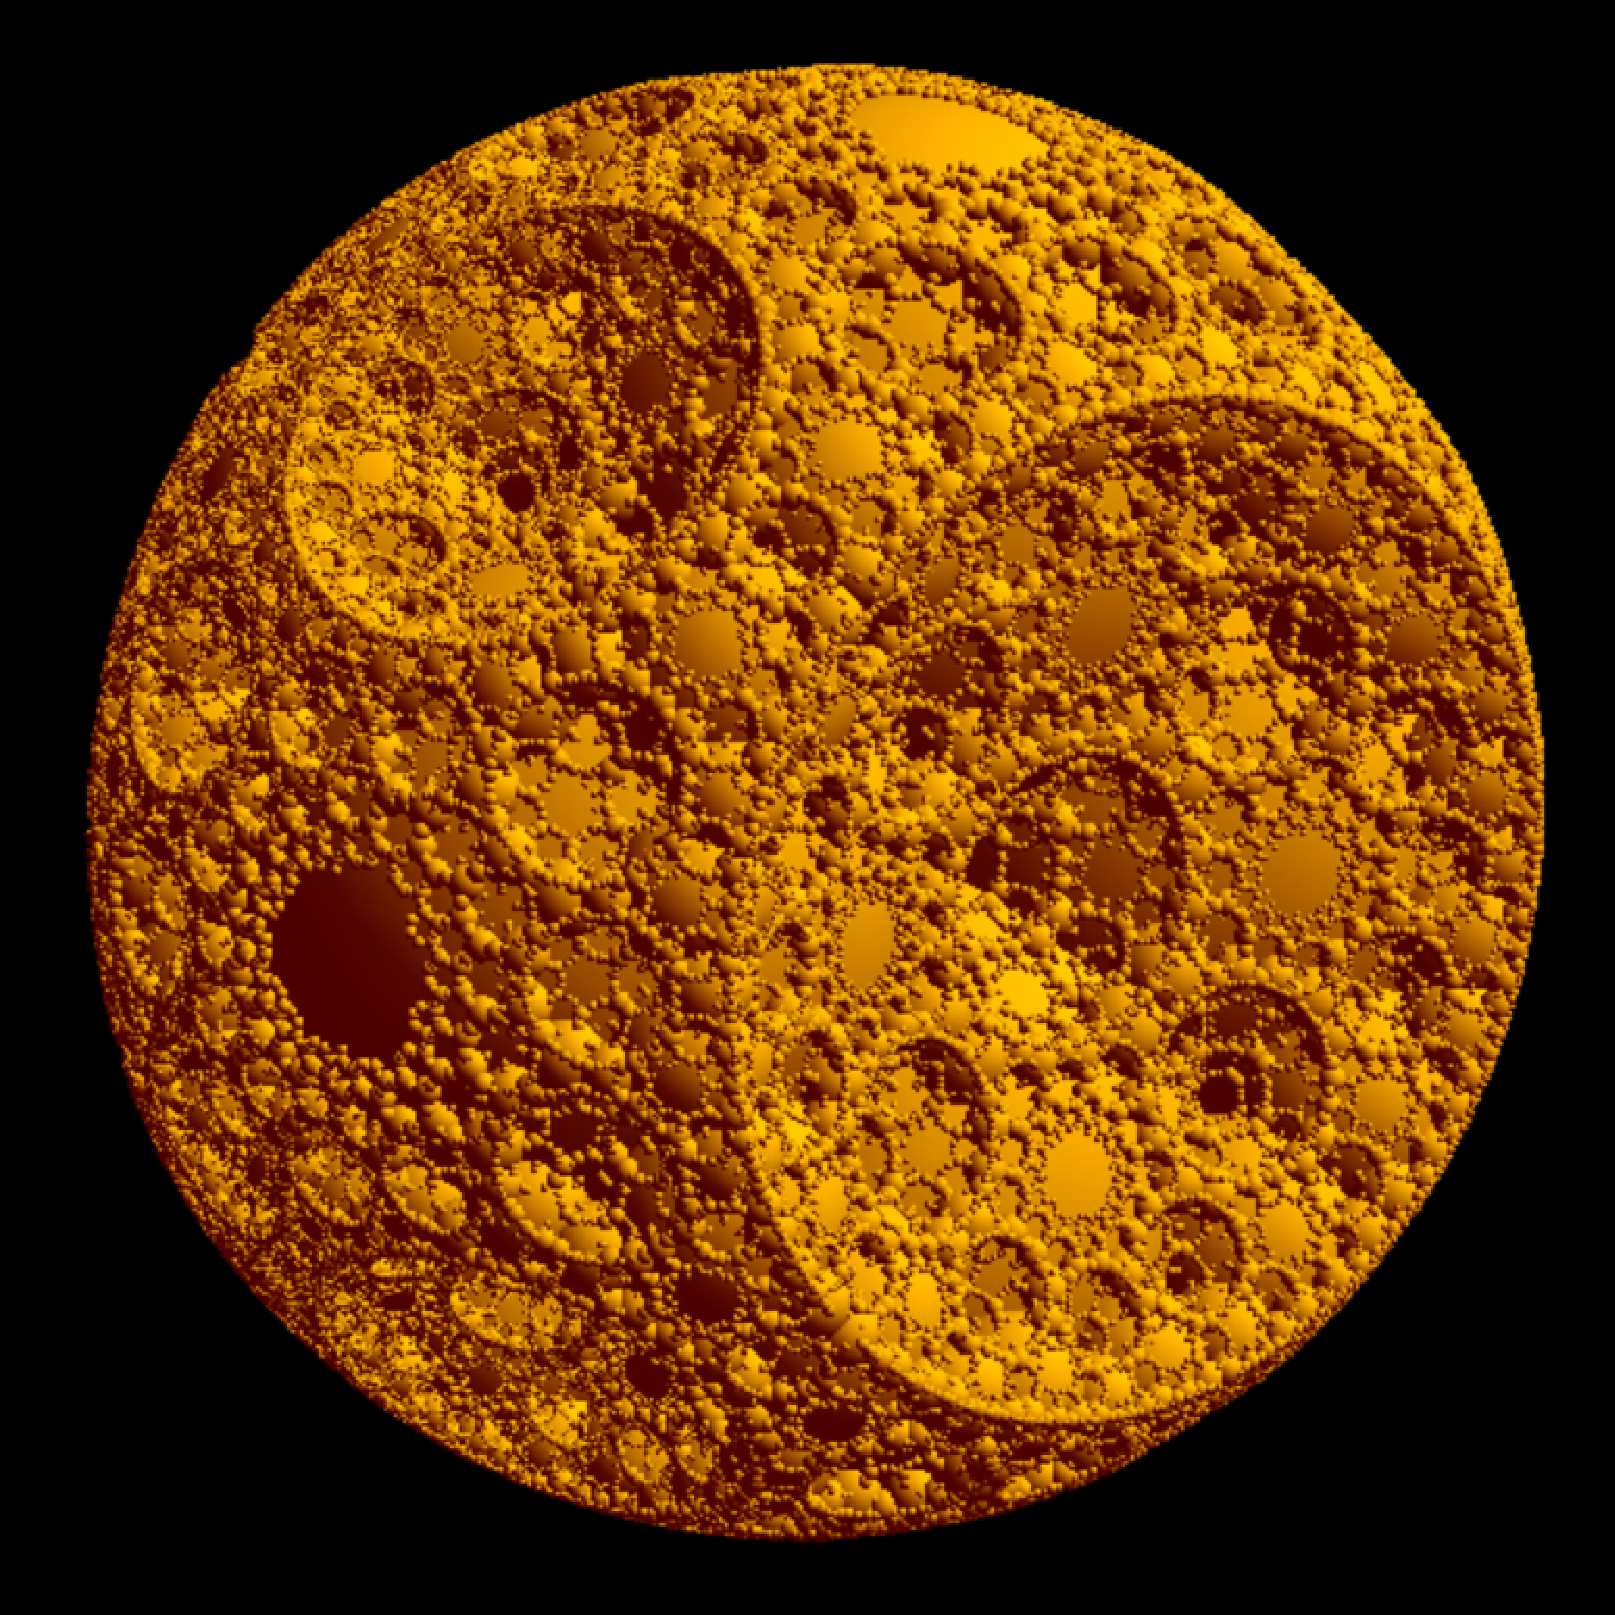
\includegraphics[width=3in, height=3in, keepaspectratio]{../img/klein/quasi-fuchsian.pdf}
   \caption{quasi-fuchsian}
   \label{fig:quasiFuchsian}
  \end{center}
 \end{minipage}
\end{figure}

\subsubsection{Other 4-Dimensional Kleinian Groups}

インドラの真珠で紹介されるクライン群は複素平面にのみ作用するメビウス変換から構成されている.
現在このようなクライン群は, ほぼ研究され尽されてしまった.

しかし, 四元数を用いることで,三次元空間に作用するメビウス変換を定義することができる.
これは$sp^k(1, 1)$と呼ばれ,2x2の四元数行列で表現される.
三次元空間上で捩じりが加わるようなメビウス変換は \emph{複合放物型}({\it
Compund Parabolic}), \emph{複合斜航型}({\it Compound Loxodromic})と分類
される.

四元数で構成されるメビウス変換とその分類は佐久川による
\cite{sakugawaMaster}や\cite{accidentalParabolic}にまとまっている.

図\ref{fig:sakugawa}は佐久川氏による複合放物型変換を含む群のレシピによる群の極限集合を描画したものである.
放物型変換である平行移動に回転が加わることで複合放物型変換となる.

荒木・糸両氏はマスキット群を四次元クライン群に拡張した\cite{maskit}.
幾何学的性質をうまく使うことで,四元数の計算を避けている.
レンダリングされた極限集合は糸氏のWebページ\footnote{4-dimensional
Kleinian punctured torus groups:
\url{http://www.math.nagoya-u.ac.jp/~itoken/3d-maskit/3d-maskit.html}}や
論文中で見ることができる.佐久川氏はこの群の四元数表示を導出した
\cite{sakugawa4d}.

三浦氏は3つ以上の生成元による4次元クライン群をモジュラー群から構成することを試みた\cite{miura}.筆者はこの論文における数値実験と可視化を行った.

\begin{figure}[h!tbp]
 \begin{subfigure}{0.49\hsize}
   \begin{center}
    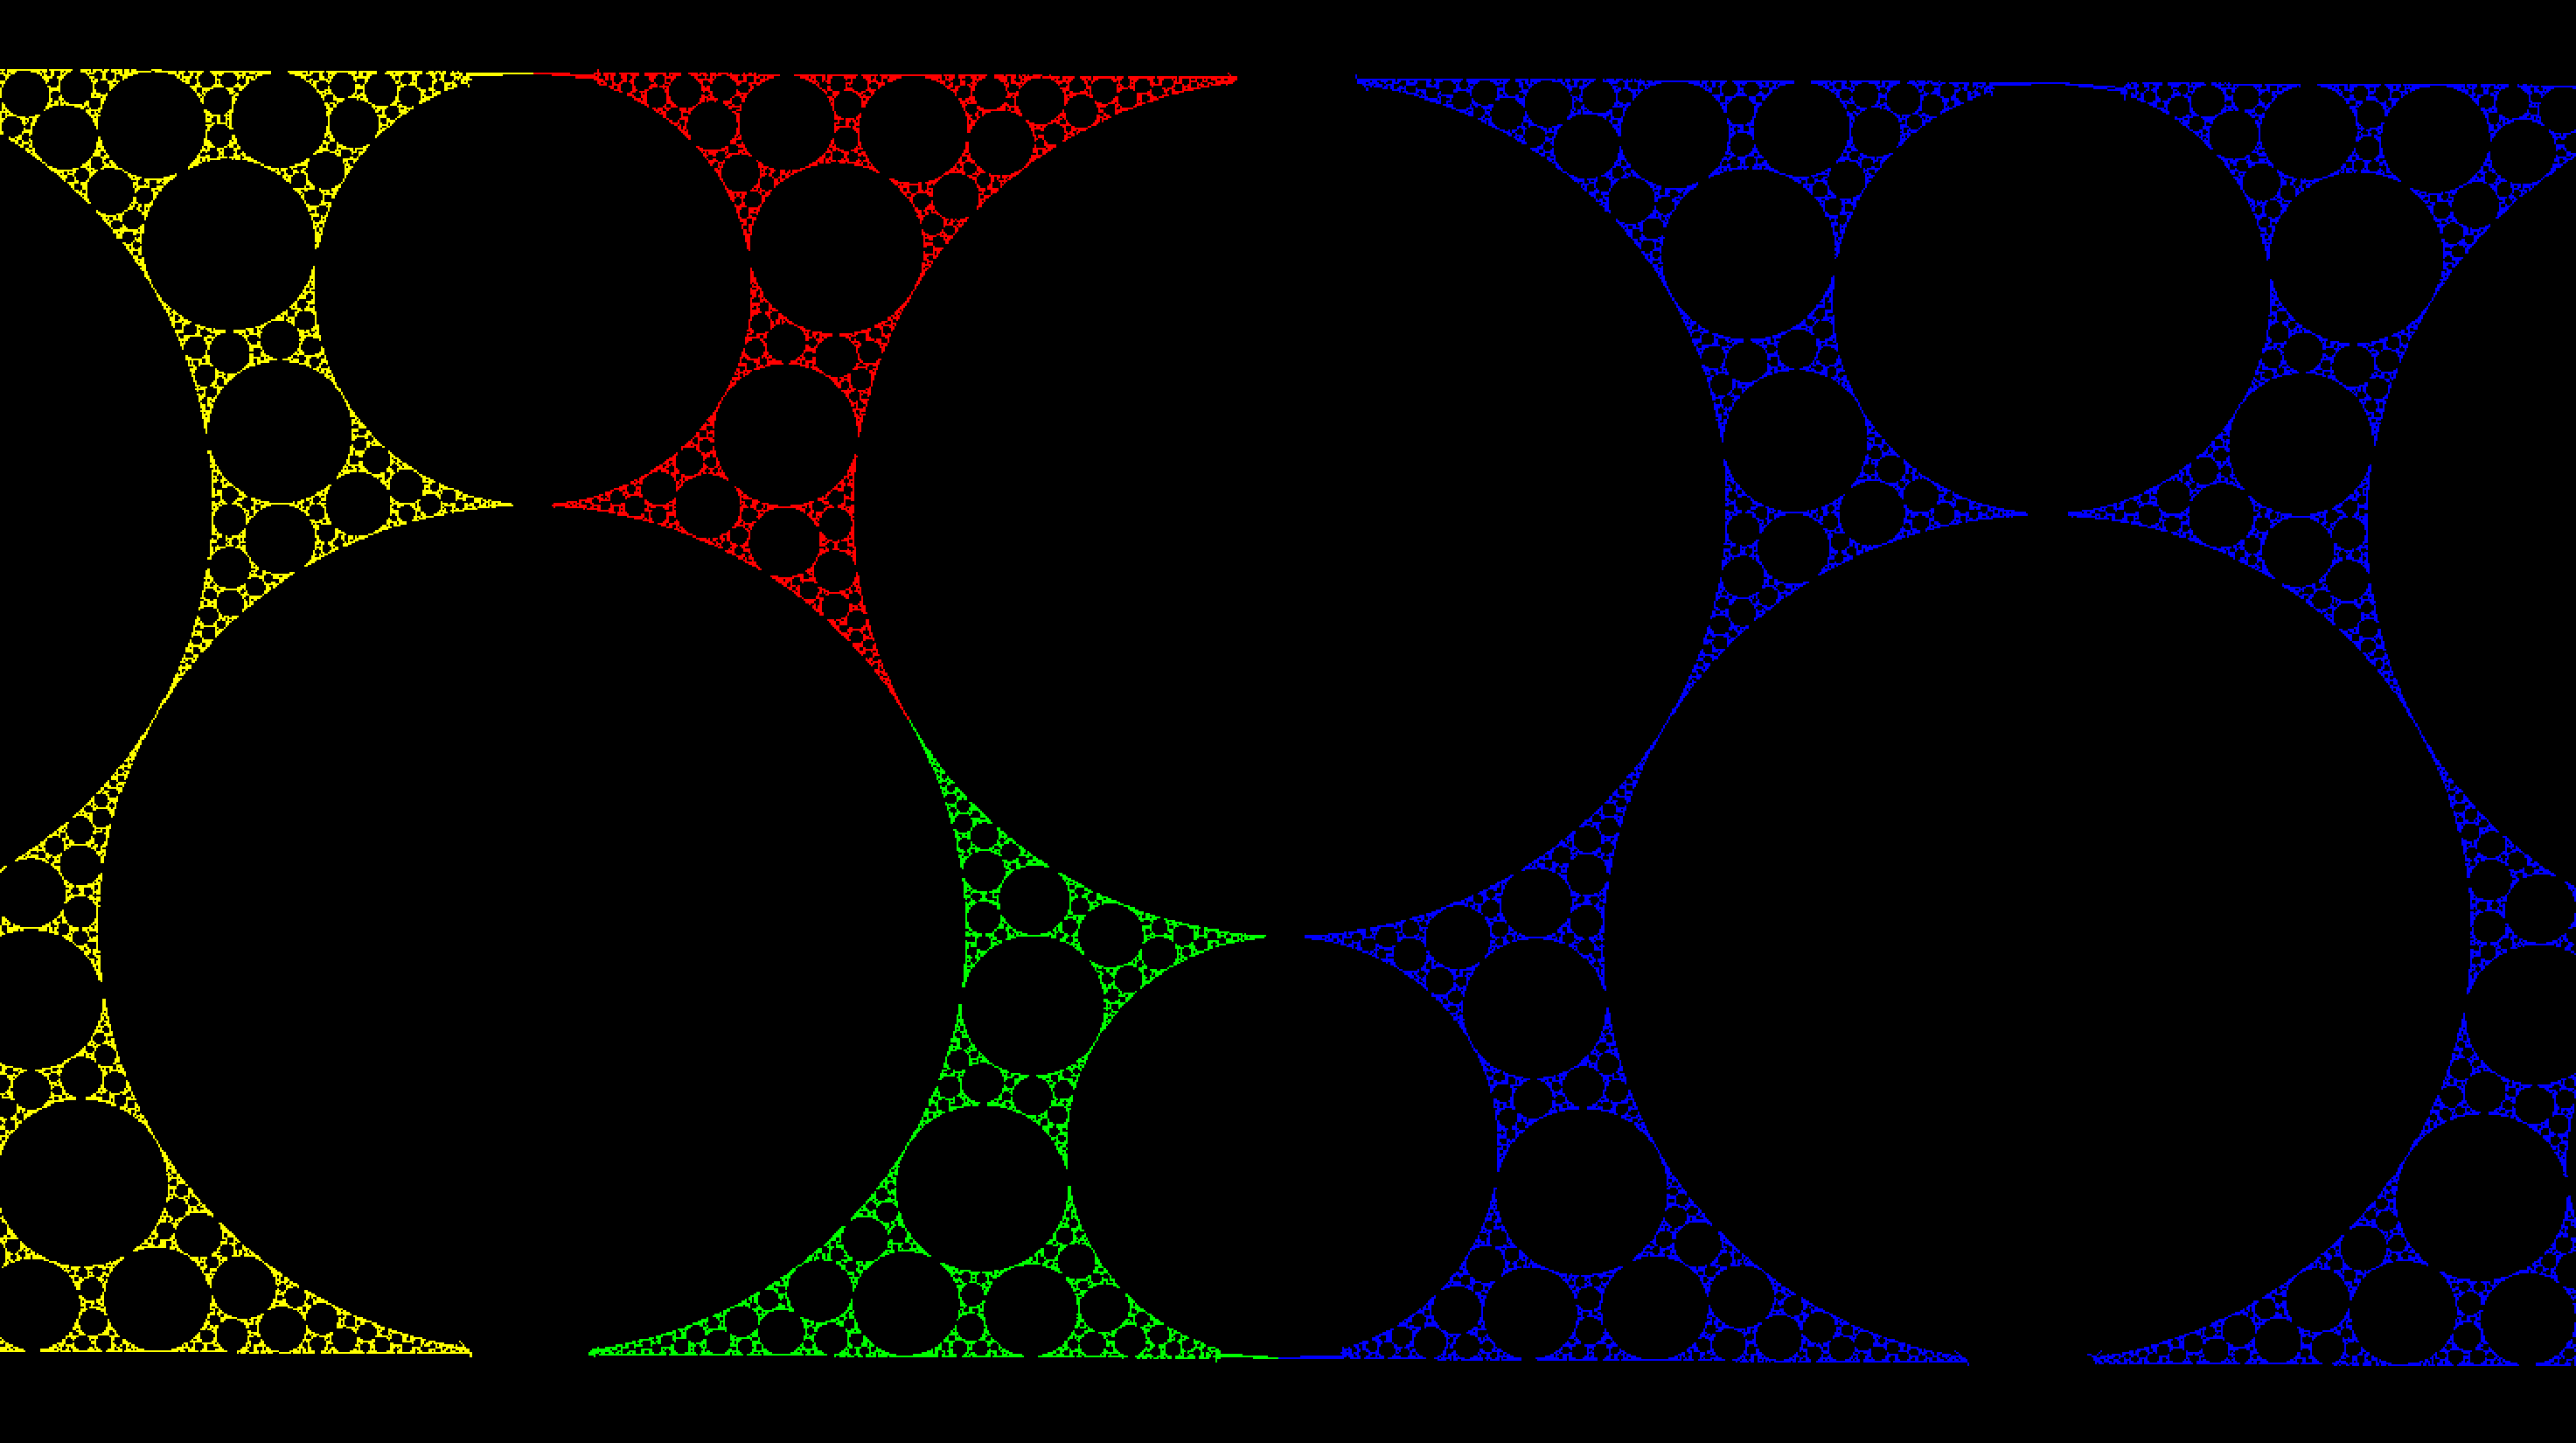
\includegraphics[width=3in, height=3in, keepaspectratio]{../img/klein/sakugawa1.pdf}
    \caption{}
    \label{fig:sakugawa1}
   \end{center}
 \end{subfigure}
 \hspace*{\fill}
 \begin{subfigure}{0.49\hsize}
   \begin{center}
    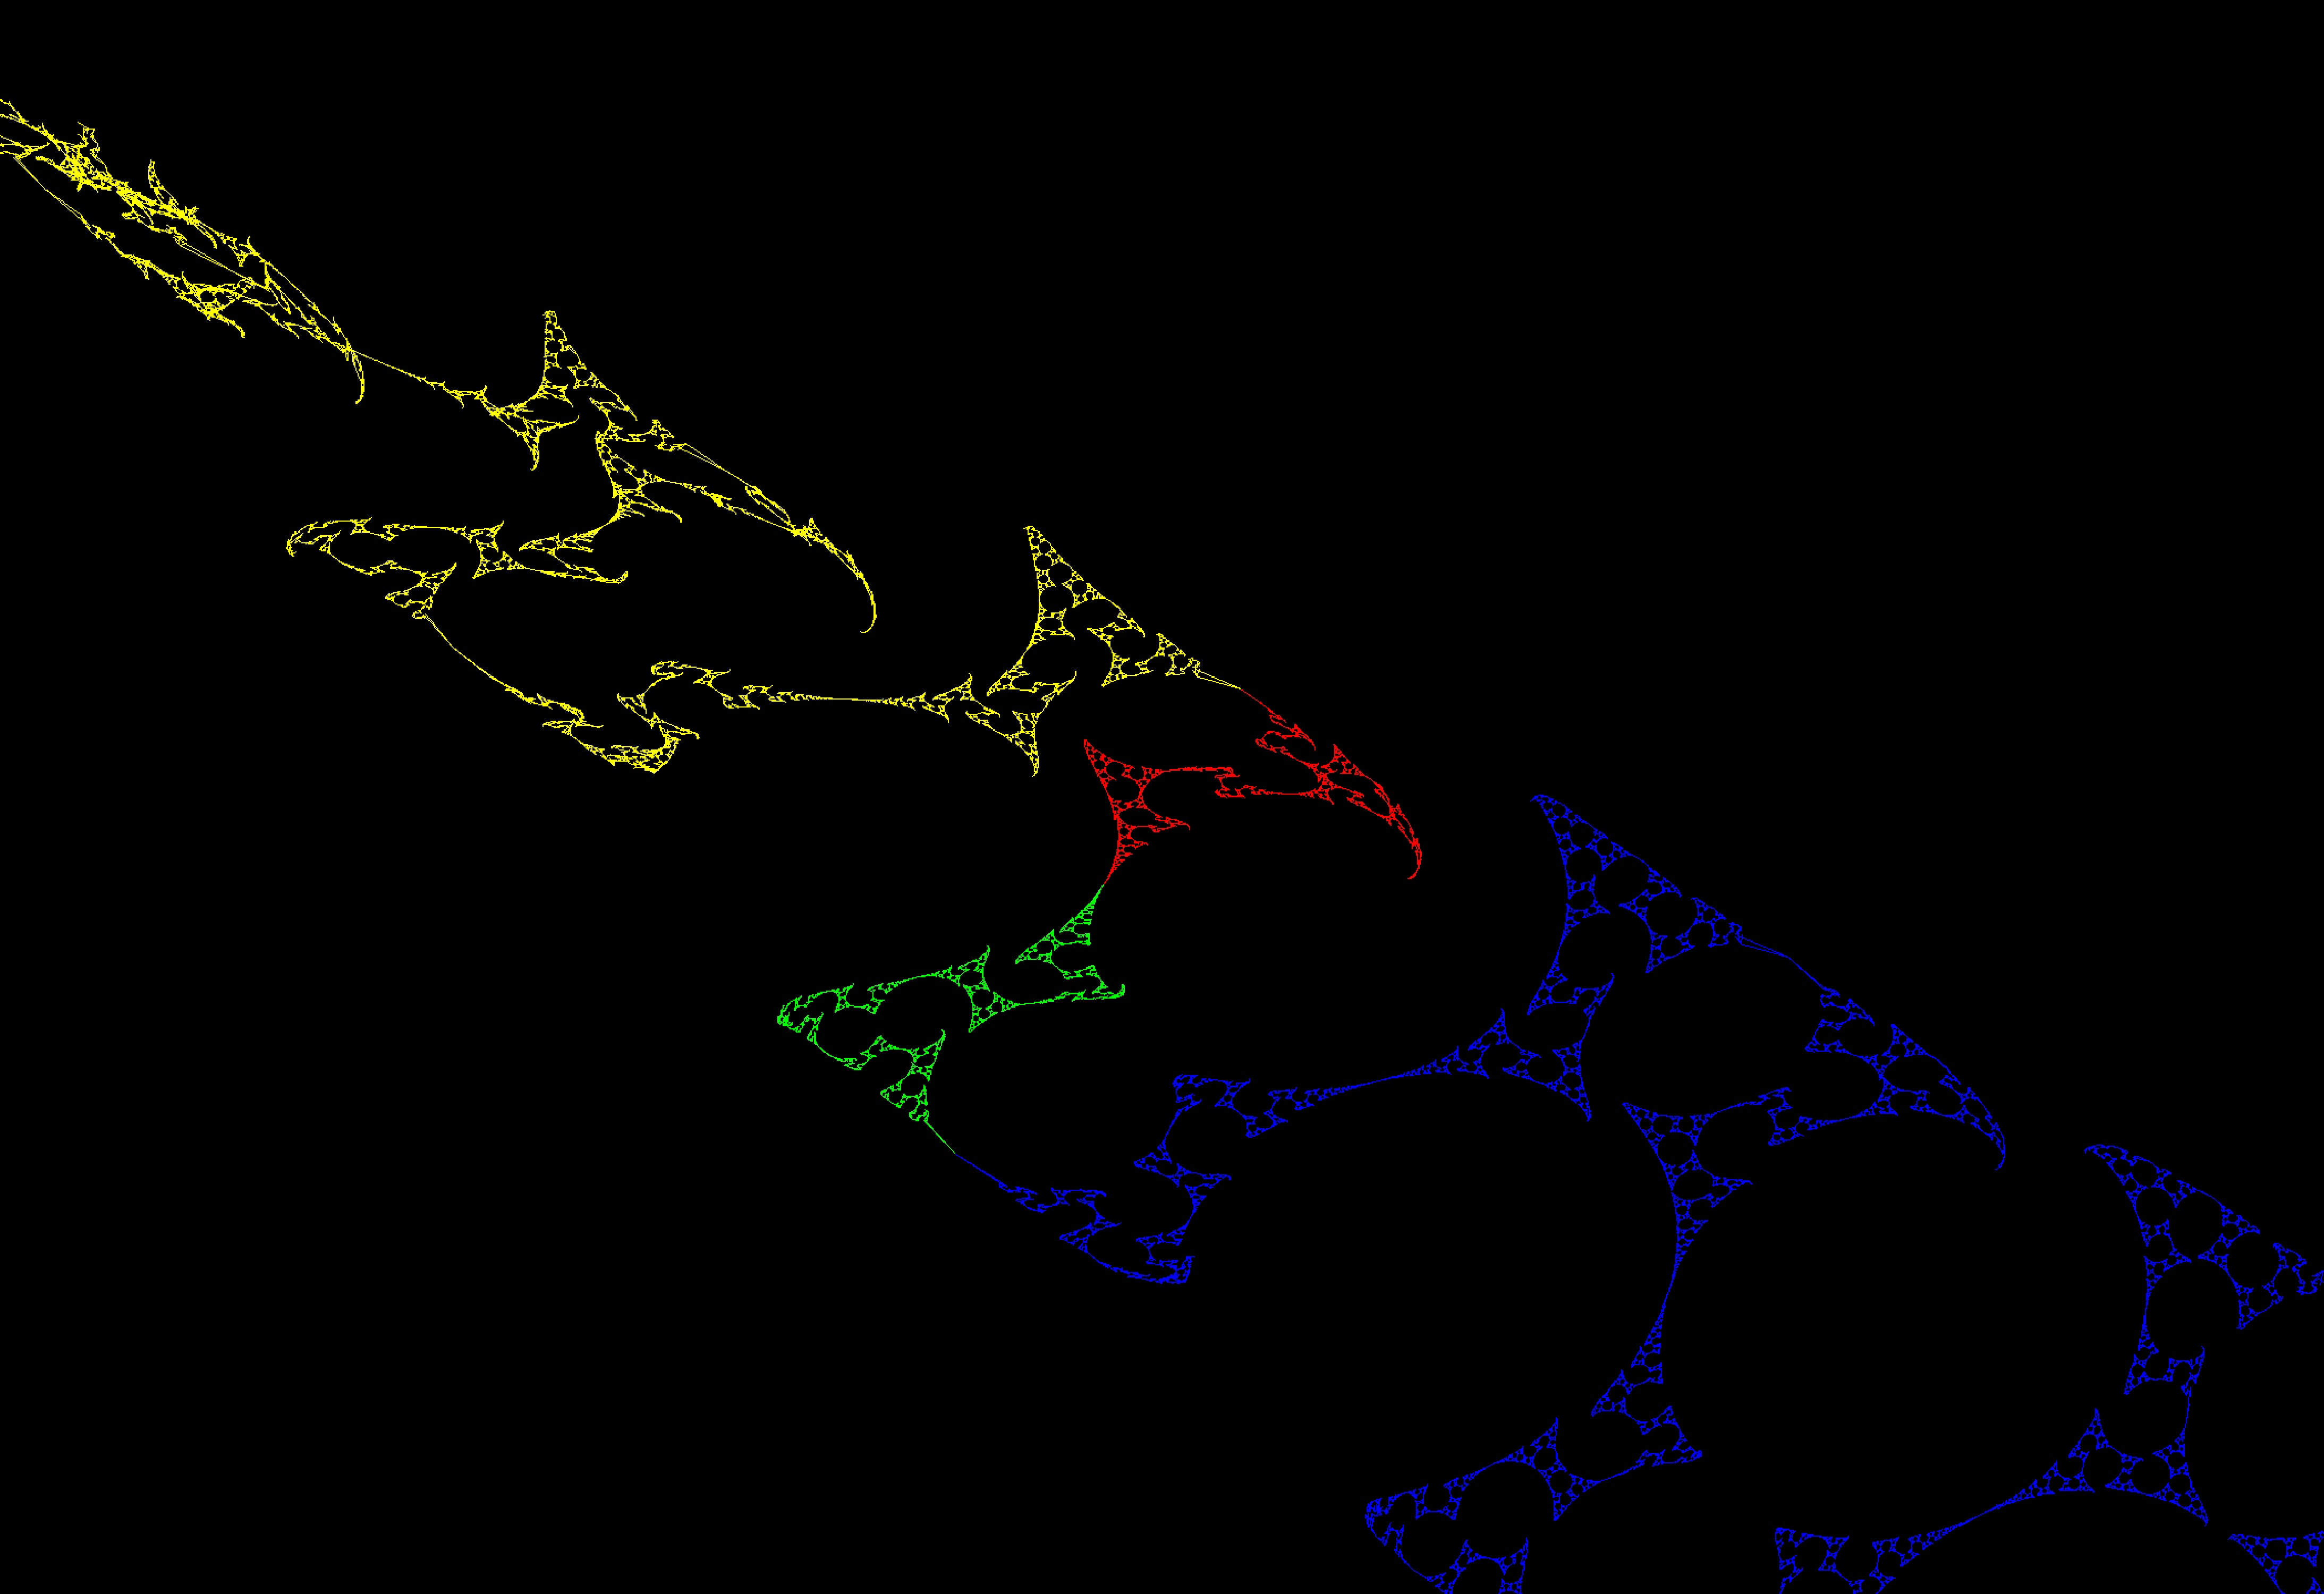
\includegraphics[width=3in, height=3in, keepaspectratio]{../img/klein/sakugawa2.pdf}
    \caption{}
    \label{fig:sakugawa2}
   \end{center}
 \end{subfigure}
 \caption{The limit set of the 4-Dimensional Kleinian Groups}
 \label{fig:sakugawa}
\end{figure}

\subsubsection{Once Punctured Torus Groups}
{\it Once Punctured Torus Groups}はクライン群の一種である.
{\it OPTi}\footnote{OPTi: \url{http://delta-mat.ist.osaka-u.ac.jp/OPTi/index.html}}という描画ソフトウェアが有名である.
描画\cite{OPTiDrawing}や離散性判定\cite{OPTiDiscrete}のためのアルゴリズムが和田によりまとめられている.
このスライス領域はベアズスライスとよばれる.
Once Punctured Torus Groupsの研究はOPTiによって進歩した.
図\ref{fig:opt}のように, 平行移動の生成元をもつため, 極限集合は比較的高速に描画することができる.

\begin{figure}[htbp]
 \begin{center}
      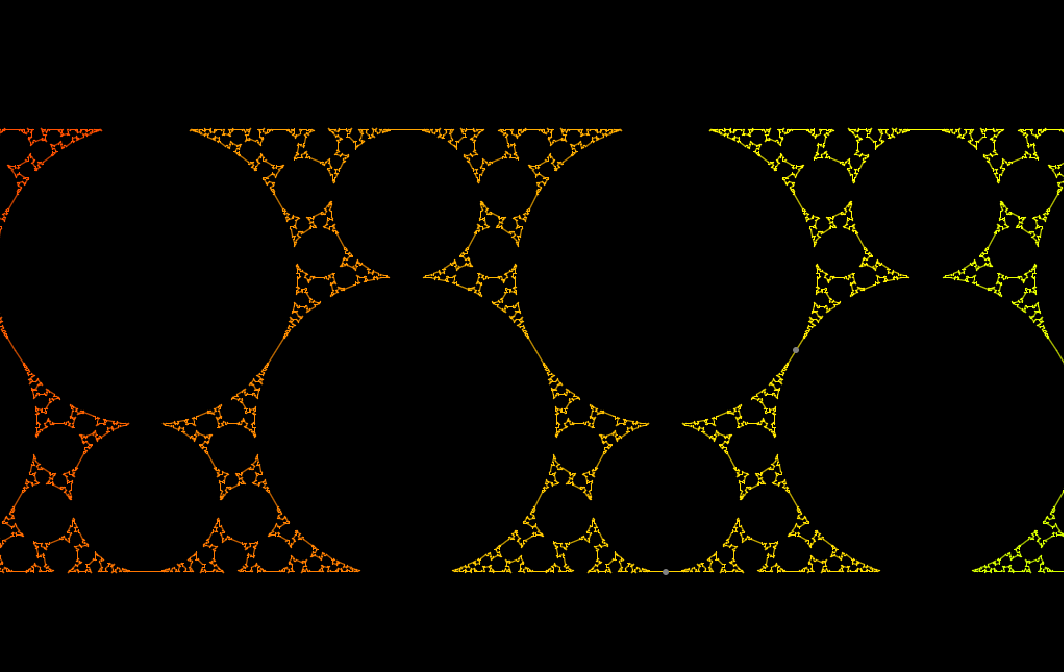
\includegraphics[width=3in, height=3in, keepaspectratio]{../img/klein/optg.pdf}
    \caption{The Limit Set of the once punctured torus groups}
    \label{fig:opt}
 \end{center}
\end{figure}

\subsection{Further Readings}
この章の最後に,クライン群のより数学的な背景を学習するための書籍をいくつか挙げておく.
『双曲幾何学への招待』\cite{invitation}は絶版であるが双曲幾何学の基本事項がまとまっている.
クライン群のより数学的内容に踏み込んだ書籍には『双曲多様体とクライン群』\cite{manifold}や『Outer Circles』\cite{outerCircles}がある.
また, レクチャーノート集に『Kleinian Group and Hyperbolic 3-Manifolds』\cite{kleinianGroupsAndHyperbolic3-Manifolds}や
『Spaces of Kleinian Groups』\cite{space}がある.
